

\subsection{Estimating root locations}

For various reasons, not all ARGs have a single root, often identified as the GMRCA. In these scenarios, we can use a generalized version Equation 2 from \cite{Osmond2021} to estimate the locations of these multiple roots, conditional on the locations of the samples, $L_s$, and the covariance matrix between the paths to the samples, $\Sigma_{(ss)}$.

As there may be multiple paths from a given sample to the root, the column vector, $L_s$ of size $n$ x 1, will need to be expanded to match the size and ordering of paths within $\Sigma_{(ss)}$. Let $P$ be a lookup matrix of size $p$ x $n$, where position $i,j$ in $S$ has value 1 if path $i$ starts at sample $j$, otherwise this position has value 0. We create a path locations column vector, $L_p$, by converting the sample locations column vector using $L_p=PL_s$, where $L_p$ has size $p$ x 1.

Let $R_s$ is be a lookup matrix of size $r$ x $p$, where $r$ is the number of roots in the tree sequence. Position $i,j$ in $R_s$ has value 1 if path $j$ terminates at root $i$, otherwise this position has value 0.

\begin{equation}
    \label{eq:location_of_roots}
    A = R_s\Sigma_{(ss)}^{-1}R_s^T
\end{equation}

\begin{equation}
    b = R_s\Sigma_{(ss)}^{-1}L_p
\end{equation}

If $\widehat{\mu}$ are root locations, we rearrange $\widehat{\mu}=A^{-1}b$ to $A\widehat{\mu}=b$ and solve for $\widehat{\mu}$ by calculating the reduced row echelon form of the augmented matrix $[A|b]$. This returns a vector containing the maximum likelihood estimates for the tree sequence root locations given the sample locations and shared time between paths.


\subsection{Calculating the covariances between lineages given an ancestral recombination graph}

In a phylogenetic tree, each sample is associated with a single path (lineage) connecting it back to the root of the tree. Samples within an ARG may be associated with multiple paths if they are found beneath a recombination node. The number of paths that connect samples nodes to the GMRCA is dependent on the number and location of recombination nodes within the ARG. We calculate the covariance between paths in the ARG as the sum of edge lengths that they share. The values are stored as a matrix, $\Sigma_{(ss)}$, with size $p$ x $p$, where $p$ is the number of paths from samples nodes to the GMRCA. The subscript $(ss)$ denotes that this is a covariance matrix between all of the paths that lead to sample nodes; this will be an important distinction in later methods, though can be ignored at the moment. Below we describe two methods for efficiently calculating this matrix: paths and bottom-up. Importantly, both methods result in the same covariance matrix, though they perform this calculation in different ways.



\subsection{Terminology}


We define a full ARG as a directed acyclic graph with each node corresponding to a haploid genome after meiosis (NOTE: {\tt tskit} records the haploid genome before meiosis, which is why recombination events are marked by two nodes). In a diploid population, each individual corresponds to two nodes in the graph. Every edge is directed from a child node to its parent node, where a node can be one of the following:
\begin{itemize}
    \item Sample node, which has no child nodes and one parent node.
    \item Coalescent node, which has two or more child nodes and one parent node. (NOTE: The methods holds for multiple merger events as well which have more than two child nodes.)
    \item Recombination node, which has two parent nodes and a child node. This is also present in the individual within which recombination happens. (NOTE: Since {\tt tskit} stores haploid genomes before recombination, it records two separate nodes belonging to the same individual for each recombination event, which have the same child node.)
    \item Root node, which has no parent and a single child. 
    \item Truly unary node, which has one parent and one child node. (NOTE: This is a subset of the unary nodes as defined in {\tt tskit}.)
\end{itemize}

Any node that isn't a sample node is called an internal node. Further, each node is associated with a time such that edges can only go from an older node to a younger node. The time associated with a node $v$ is denoted by $t_v$ . We define a simplified ARG as one without the truly unary nodes. Throughout the text, we deal with a simplified ARG. This is distinct from a {\tt tskit} simplified tree sequence since truly unary nodes are only a subset of the unary nodes and {\tt tskit} simplify also involves other simplification steps. We don't make any assumption about non-ancestral nodes and edges but talk about their effects later. 



In order to infer dispersal rates and ancestral locations from locations of present day samples, we assume we have the simplified ARG of the samples, as defined above.  Such an ARG can be obtained from {\tt ARGweaver}, {\tt KwARG} or {\tt ARGinfer}.



\section{Methods}

\subsection{Multiple roots}

Since the Brownian motion assumption doesn't hold in the deeper past due to finite habitats \citep{Ianni2022, WakeleySCATTERINGETC} and inference until the GMRCA isn't usually desirable or possible from the sequence data \cite{}, we will often want to cut off an ARG some time in the past. 
Doing this often results in the ARG having multiple roots, which hasn't been accounted for above. Let $\vec{\mu}$ be the vector of root locations. The likelihood function is then given by 
\begin{eqnarray}
    p_{\Lvec}(\lvec \ ) = \frac{ \text{exp} [ -\frac{1}{2\sigma^2} (\Pp\lvec - \Rp\muvec)^\text{T} \spathg (\Pp\lvec - \Rp\muvec) ] }{\sqrt{ (2\pi\sigma^2)^n |\spath|  }}
\end{eqnarray}
where $\Rp$ is a lookup matrix of size $p \times r$, with $r$ being the number of roots in the ARG. Position $i,j$ in $\Rp$ has value 1 if path $i$ contains root $j$, and 0 otherwise. 

NOTE: The full covariance between the paths is $\sigma^2 ( \spath + [ \text{Cov}( (\Rp\muvec)_i, (\Rp\muvec)_j ) ] )$. However, because we assume that the root locations are independent of each other and constant, the second term in zero. Since, in practice, we cut off the trees at a point by which the ancestors are well mixed in a finite habitat, the assumption of independence is reasonable. (The constant assumption could be relaxed by adding the variance of a uniform distribution over the habitat to the diagonal blocks.) 

We can then compute the maximum likelihood estimate for the root locations, given the sample locations, $\ldata$, as a solution to the following system of linear equations

\begin{eqnarray}
    \label{eq:location_of_roots}
    \mathbf{A} \muvecMLE = \vec{b} 
\end{eqnarray}
where 
\begin{eqnarray}
    \mathbf{A} &=& \Rp^\text{T}\spathg\Rp  \\
    \vec{b} &=& \Rp\spathg\Pp\ldata
\end{eqnarray}
If $\mathbf{A}$ is invertible (NOTE: Haven't proved it but I think this should always be invertible), then there exists a unique solution,
\begin{eqnarray}
 \muvecMLE = (\Rp^\text{T}\spathg\Rp)^{-1} \Rp\spathg\Pp\ldata   
\end{eqnarray}
which is a generalized version of $\muMLE$ (above) and reduces to the same form for a single root (in which case $\Rp = \onevec{p}$).

Once we have the roots, we can compute the unbiased estimator for the dispersal rate as before 
\begin{eqnarray}
    \sigmaMLE &=& \displaystyle \frac{ (\Pp\ldata - \Rp\muvecMLE)^\text{T} \spathg (\Pp\ldata - \Rp\muvecMLE) }{n-k}.
\end{eqnarray}
where $k = \text{trace}[  \Pp^\text{T}\spathg\Rp(\Rp^\text{T}\spathg\Rp)^{-1}\Rp^\text{T}\spathg\Pp(\Pp^\text{T}\spathg\Pp)^{-1} ]$. The $n-k$ is the correction for the bias in the Maximum Likelihood Estimator (See Appendix \ref{}), which depends on the topology and branch lengths of the ARG. When there is a single root ($\Rp = \onevec{p}$) then $k=1$ (as above), which is the same as for a tree.

\subsection{Internal Node Locations}
  

Once we have the estimates of the dispersal rates and root locations, we can get the distribution of internal node locations as well. Given an internal node, $a$, its location, $\Lint$ is distributed as
\begin{eqnarray}
    \Lint | \muvecMLE, \sigmaMLE, \ldata \sim \cN( \muMLE_a + \savec^\text{T}\spathg(\Pp\ldata - \Rp \muvecMLE), \sigmaMLE(t_a - \savec^\text{T}\spathg\savec))
\end{eqnarray}
conditional on the dispersal rate, root locations, and observed sample locations. However, since the root locations have associated uncertainty, one can use the law of total variance to find the complete variance,
\begin{eqnarray}
    \Var \Lint = \sigmaMLE\left(t_a - \savec^\text{T}\spathg\savec + \displaystyle \frac{(1 - \savec^\text{T}\spathg\onevec{p})^2}{\onevec{p}^\text{T}\spathg\onevec{p}}\right).
\end{eqnarray}

\subsection{Mean Centering}

For a genealogical tree, the unbiased dispersal estimate and the distribution of internal node locations can be computed without estimating the root location. This is done through mean-centering the observed locations (Eq 12, 24 and 25 of \cite{Osmond2021}), where the mean sample location is substracted from each sample location and dropping a sample. To extend the method to ARGs, we need to subtract the mean of the path locations (which would be a weighted average of the sample locations) instead of the mean of sample locations. 

\subsubsection*{A Single Root}

In the case that the ARG has a single root, the Grand Most Recent Common Ancestor (GMRCA), mean-centering is done by subtracting the mean sample location over all paths from the sample location of each path, and dropping all paths associated with a sample. The mean-centered locations and covariance matrix are given by $\xvec = \Mp \lpvec $ and $\sigma^2 \Vp = \sigma^2 \Mp \spath \Mp^\text{T}$ where $\lpvec= \Pp \lvec$ (NOTE: Didn't think this notation was needed until here) and $\Mp$ is a $p \times p-p_n$ matrix with $1 - \displaystyle \frac{1}{n}$ on the diagonal entries and $\displaystyle -\frac{1}{n}$ everywhere else (NOTE: This is true if all the paths form the last sample are at the end. Need to figure out when that is not the case). Here $p_n$ are the number of paths associated with the last sample. Then the dispersal estimate and the distribution of an internal node location are given by 
\begin{eqnarray}
    \sigmaMLE &=& \displaystyle \frac{ \xdata^\text{T} \Vp \xdata }{n-1} \\
    \Lint &\sim& (\bar{L_p} + ) 
\end{eqnarray}

\subsubsection*{Multiple Roots} 

NOTE: Need to figure out notation for this. So this description is still informal. New Notations and redundancies might exist

Let $P_i$ be the set of indices of the paths associated with the $i^\text{th}$ root. Then mean-centering would involve subtracting from the path locations in $P_i$ their mean. Therefore if two paths from the same sample go to different roots, the corresponding path locations would be mean-centered using different means. Then as before the 


 
\subsection{Algorithm}

\begin{figure}[htp]
    \centering
    \includegraphics[width=12cm]{Images/algorithm.png}
    \caption{Visualization of the optimized algorithm. Given a hypothetical ARG of three samples (left) with four paths, the algorithm builds the covariance matrix by looping through the nodes in the ARG. Within the looping block, the bolded numbers in each matrix are those that were updated in that specific step.}
    \label{fig:algorithm}
\end{figure}


\begin{figure}[h]
    \centering
    \includegraphics[width=0.45 \linewidth]{Images/AlgorithmEfficiency.jpg}
    \caption{Benchmarking for the time that it took the each methods to calculate the shared time matrices, $\spath$, for a set of random ARGs generated by the msprime Python package \citep{Baumdicker2022}. More details on the parameters passed to msprime can be found in the Supplementary. Both algorithms were run on the same set of ARGs, and for each ARG, the algorithm that went first was chosen at random to minimize any unintended biases associated with the ordering of the algorithms.}
    \label{fig:AlgorithmEff}
\end{figure}

The key object for computing dispersal rates and node locations is the matrix of shared time between paths, $\spath$. One can use existing methods in {\tt Python} to find each path from the samples to the GMRCA and then find the intersection between different paths to compute the entries of the shared time matrix. However, this doesn't scale well to larger ARGs. A primary reason for the exponential increase in time is the common edges between different paths. For instance, the edges marked in red in Fig \ref{fig:AlgorithmEff} will be traversed at least twice when finding the unique paths. By developing an algorithm that traverses each edge only once, we were able to speed up the process, allowing the method to be applied to larger ARGs (Fig \ref{fig:AlgorithmEff}). Briefly, the algorithm entails an bottom-up traversal of the ARG starting at the sample nodes and updating the matrix as we traverse upwards towards the roots. Here we present an outline of the algorithm (see end of Appendix \ref{appedix:ch2} for a step-by-step implementation of the algorithm for a simple ARG). 

\begin{enumerate}
    \item Initialization 
    \begin{itemize}
        \item The shared time matrix $\mathbf{S} = [0]_{n \times n}$, a zero square matrix of size $n$, the number of samples.
        \item The set of current nodes CN $= \{1,2,...,n \}$ with the sample nodes.
        \item The list of paths PL $= [ [1], [2],..., [n]  ] $ with one path for each sample node. 
    \end{itemize}
    \item From CN, choose the oldest node, say $o$. Let $I_o$ be the set of indices of the paths in PL that end in $o$. Let $k_o$ be the the number of parent nodes of $o$. 
    \begin{enumerate}
        \item If $k_o=0$, skip this step. 
        \item If $k_o=1$, with parent node $x$, add $t_{xo}$ to all $s_{ij}$ where $i,j$ are in $I_0$. Append $x$ to all the paths that currently end at $o$.
        This step is extending the paths that till this point ended at $o$ to $x$. Since they all will share the edge $ox$, we add it to the corresponding covariance terms.
        \item If $k_o=2$, with parent nodes $x_1$ and $x_2$, duplicate all the columns and rows of $\mathbf{S}$ with indices in $I_0$, as well as the corresponding paths in PL. Let the indices of the duplicated rows and columns be $I_{new}$. Add $t_{ox_1}$ to all $\mathbf{S}_{ij}$ such that $i,j$ are in $I_0$ and add $t_{ox_2}$ to all $\mathbf{S}_{ij}$ such that $i,j$ such that $i,j$ are in $I_{new}$. Append the paths at indices in $I_o$ with $x_1$ and the paths at indices in $I_{new}$ with $x_2$
    \end{enumerate}
    \item Delete $o$ from the set of current nodes, CN, and add the parent nodes ($\{\}$, $\{x\}$, or $\{x_1,x_2\}$) to it. 
    \item Repeat Steps 2 to 4 until CN only has root nodes in it. 
\end{enumerate}


\section{Mean Centering}

\subsection{Mean Centering}

For a genealogical tree, the unbiased dispersal estimate and the distribution of internal node locations can be computed without estimating the root location. This is done through mean-centering the observed locations (Eq 12, 24 and 25 of \cite{Osmond2021}), where the mean sample location is substracted from each sample location and dropping a sample. To extend the method to ARGs, we need to subtract the mean of the path locations (which would be a weighted average of the sample locations) instead of the mean of sample locations. 

\subsubsection*{A Single Root}

In the case that the ARG has a single root, the Grand Most Recent Common Ancestor (GMRCA), mean-centering is done by subtracting the mean sample location over all paths from the sample location of each path, and dropping all paths associated with a sample. The mean-centered locations and covariance matrix are given by $\xvec = \Mp \lpvec $ and $\sigma^2 \Vp = \sigma^2 \Mp \spath \Mp^\text{T}$ where $\lpvec= \Pp \lvec$ (NOTE: Didn't think this notation was needed until here) and $\Mp$ is a $p \times p-p_n$ matrix with $1 - \displaystyle \frac{1}{n}$ on the diagonal entries and $\displaystyle -\frac{1}{n}$ everywhere else (NOTE: This is true if all the paths form the last sample are at the end. Need to figure out when that is not the case). Here $p_n$ are the number of paths associated with the last sample. Then the dispersal estimate and the distribution of an internal node location are given by 
\begin{eqnarray}
    \sigmaMLE &=& \displaystyle \frac{ \xdata^\text{T} \Vp \xdata }{n-1} \\
    \Lint &\sim& (\bar{L_p} + ) 
\end{eqnarray}

\subsubsection*{Multiple Roots} 

NOTE: Need to figure out notation for this. So this description is still informal. New Notations and redundancies might exist

Let $P_i$ be the set of indices of the paths associated with the $i^\text{th}$ root. Then mean-centering would involve subtracting from the path locations in $P_i$ their mean. Therefore if two paths from the same sample go to different roots, the corresponding path locations would be mean-centered using different means. Then as before the 


\section{Results 2 - Old } 

\textbf{alternative outline}
\begin{itemize}
    \item dispersal rate
    \begin{itemize}
        \item composite trees: this estimate considers the trees as independent realizations of the spatial process, and effectively averages over them
        \item now condition on trees all sharing GMRCA: increases the dispersal estimate because internal nodes are moved away from minimum dispersal paths in each tree
        \item now condition on the trees meeting at the samples too (funny ARG): gives new likelihood with larger dispersal rate because of loops, ie more internal node constraints
        \item finally, condition on trees sharing edges too (full ARG): more loops/constraints, higher dispersal rates
        \item ARG estimates wrong: given that composite trees does the right thing and that adding loops increases the dispersal estimate, ARG estimate is wrong
    \end{itemize}
    \item ancestor locations
\end{itemize}

We first highlight how including correlated trees affect dispersal estimates. Even though Brownian motion leads to the issue of spatial clumping (pain in the torus ref), previous analysis have shown it to be a good approximation when ------------------- (confirm the exact conditions especially in the presence of recombination.). In particular, it works for a history without recombination. Osmond and Coop (2021) got better estimates of dispersal by taking an average of estimates over trees in a tree sequence from regions of the genome with low linkage. They assumed that due to multiple recombination events between any two of the sampled trees, that these trees shared no common ancestors. We first describe the various ways in which the estimates using the corresponding ARG (consisting only of the sampled trees) would differ. 
\begin{enumerate}
    \item First, when using the ARG, we condition on the Brownian motions meeting at the samples. This differs from the Osmond and Coop method where the movement in one tree doesn't affect movement along another tree. However, the Osmond and Coop method would be equivalent to the "incorrect" likelihood function that we are using if the trees indeed didn't share any common ancestors. 
    \item Apart from meeting at the samples, the different trees also share the GMRCA and hence start at the same point. When considering any single tree, the MLE estimates of the MRCA is such that it minimizes the dispersal rate for that tree. However, having the same GMRCA for multiple trees, would necessarily mean deviating from the minimal dispersal path for each tree, thereby increasing the dispersal rate. 
    \item Finally, apart from the the samples and the GMRCA, these trees also share internal nodes. As in the case of accounting for the GMRCA, allowing for shared internal nodes between trees, also means deviating from the minimal dispersal path. In particular, the location for a shared internal node that minimizes dispersal in one tree wouldn't be the same location that minimizes dispersal along another.
\end{enumerate}

Therefore, the dispersal estimate from the ARG always tends to be higher than from the marginal trees. This creates a "surprising"(?) effect of the dispersal estimates increasing as we include more trees in an ARG. 



\section{Results - Old}

Outline 
\begin{itemize}
    \item Effect of a recombination loop (Fig 1)
    
    \begin{itemize}
        \item Given the same height, a recombination event increases dispersal estimate. Further, increasing the loop size increases dispersal estimate.
        \item Locations skew towards the sample which has experienced the recombination event in its history.
    \end{itemize}
    \item This method captures both the effect of branch length and correlation between adjacent trees. (Fig 2)
    \item Comparison to other methods (Fig 2)  
    \begin{itemize}
        \item Osmond and Coop - The comparison is via marginal trees estimate. Doesn't capture the correlation between marginal trees.
        \item Wilder-Wohns - Doesn't capture the branch length
        \item Modified Wilder Wohns - Doesn't capture the Correlations. 
    \end{itemize}
    \item Internal Node Locations (Fig 3)
    \begin{itemize}
        \item Intuition on what factors affect the locations (recombination nodes v/s coalescent nodes) 
        \item Effect of multiple roots. 
    \end{itemize}

    \item SliM Results
    \begin{itemize}
        \item Accuracy?  (Fig 4) - histogram of dispersal rate estimates for various subsets of samples? internal node positions with error bars versus the true locations
        \item Effect of including more trees (genome) (Fig 5) 
    \end{itemize}

    \item Effect of different steps of ARG simplification process (Fig 6) 
    \begin{itemize}
        \item Removal of recombination nodes 
        \item Removal of non-ancestral coalescent nodes 
        \item Disconnecting tree roots. 
    \end{itemize}
\end{itemize}


\begin{figure}[h]
    \centering
    \includegraphics[width=\linewidth]{Images/CompoundARGEstimates.jpg}
    \caption{(A.) The dispersal estimate and (B.) GMRCA location estimate using different methods for the ARGs. The x-axis varies the length of the loop and the ARG is depicted in the diagram. The observed location of sample 1 is -0.5 and sample 2 is 0.5}
    \label{fig:Bubble}
\end{figure}

We highlight some key ways in which accounting for recombination events can alter the estimates of dispersal and the GMRCA locations. In other words, we present the building blocks to answer how do these estimates change as we include longer genomes (of the same sample individuals) in our inference. We applied our method alongside two other alternative methods for estimating dispersal rates and/or ancestral locations on a simple ARG with three samples with $L_s=[0,0.5,1]^T$. These alternative methods were inspired by those used in previous studies, though we did not directly implement their specific methods directly (osmondestimating2021,wohnsunified2022).

Knowing that a recombination event occurred means that two lineages that had started diverging in the past came together. Since the lineages are moving randomly in space, they are more likely to come together if they didn't move too far away from where they started. Mathematically, conditioning on two independent Brownian motions meeting at the recombination node, reduces the variance in the distribution of its location, increasing the probability of the recombination node being closer to the location of the GMRCA. Therefore, for a given dispersal rate, this also reduces how far the descendants of the recombination node are expected to be from the location of the GMRCA. 
This has two key consequences for inference.
\begin{enumerate}
    \item For the same observed locations of the samples, including a linked genomic region for inference increases the dispersal estimate, provided the GMRCA remains the same. 
    \item The location of ancestors are skewed towards the sample node(s) that have experienced recombination in their history. \gc{Because....}    
\end{enumerate}

\begin{figure}[h]
    \centering
    \includegraphics[width=0.6\linewidth]{Images/StochasticARG.png}
    \caption{A plot of dispersal estimates as we include more trees from an {\tt msprime} simulated tree sequence in our analysis. The solid blue line is the dispersal estimate using our Paths method. The dotted blue line is the individual estimates from the marginal trees and the red line is the height of the tree along the sequence.}
    \label{fig:StochARG}
\end{figure}

Both of these are exemplified in Fig \ref{fig:Bubble} which computes the dispersal estimates and the location of the GMRCA for the ARG in Fig \ref{fig:Method}. For this ARG, we can see the dispersal rate estimate from the ARG is higher than that from each marginal tree. Further, the estimates of ancestral locations from the ARG are skewed towards sample one in contrast to the symmetric inference from the marginal trees.  \gc{Need to be clearer that the increasing dispersal is bc tree height is being gelps constant}
\gc{So generally this section on dispersal etc is unclear}
The dispersal estimate can also potentially decrease upon including linked regions if the \gC{which?} marginal tree is taller than all of the existing trees. This is because a taller tree means more time cover the same distance and therefore potentially a slower dispersal rate estimate. Observe in Fig \ref{fig:3samARG}.B, as we decrease the height of the shorter marginal tree (tree 1), the dispersal estimate from the ARG actually is smaller than that from the shortest tree (tree 1).
The reason the dispersal estimate does not always decrease when adding a taller tree is precisely because of linkage. Because of linkage, the two regions share many of their ancestors. Therefore the spatial movement of the lineages in the new tree need to satisfy the constraints due to the shared ancestors with existing trees. This could lead to a higher estimate of dispersal despite a taller marginal tree for the new region. In fact, we simulated the tree sequences using the {\tt msprime} package and find that usually the dispersal estimates tend to increase or stay constant as we include more trees in the analysis with the value saturating towards the end (Fig \ref{fig:StochARG}). 

\begin{figure}[h]
    \centering
    \includegraphics[width=0.25\linewidth]{Images/3samARG.jpg}
    \hspace{0.03\linewidth}
    \includegraphics[width=0.70\linewidth]{Images/3sam_compoundrecomb.jpg}
    \caption{Effect of varying different branch lengths of the given ARG on dispersal and GMRCA location estimates. A and D show the effect of varying the size of the loop without changing either of the marginal trees. B and E capture the effect of varying a branch which is part of the loop and changes the height of one of the marginal trees. C and F show the effect of changing branch lengths not contained in the loop.}
    \label{fig:3samARG}
\end{figure}

In Fig \ref{fig:3samARG}, we individually varied three critical branch lengths within the ARG (marked by the letters) and observed their effects on our estimates. We first compared the dispersal rate estimates for the ARG to the rates calculated for each of the marginal trees in the tree sequence. Importantly, the marginal tree method treats the trees independently and so ignores any correlation between neighboring trees. Each tree has its own dispersal rate, and the dispersal rate of the ARG is not a simple combination of these rates. As expected, in Fig \ref{fig:3samARG}.A, we see that the dispersal rates calculated for a marginal tree is unaffected by varying the timing of the recombination event, whereas the dispersal rates calculated from the ARG increase as the size of the loop increases.

\subsection{Application to simulated data and comparisons with alternative methods} \label{SLiMsims}

We performed simulations using SLiM 4 (hallerslim2023). Each simulation had a starting population of 10000 diploid individuals. All individuals were placed at the center of a $100 \times 100$ unit area. Each tick in the simulations corresponds with a generation. Individuals reproduce based on conditions in their local neighborhood; mates are chosen randomly based on their distance to the individual and the number of offspring is a Poisson random variable with $\lambda=\frac{R}{1 + \frac{neighbor}{K}}$. It is possible that there are no mates within the interaction distance and/or no offspring produced. Offspring are placed at random around one of their parents positions with an normally distributed offset in each dimension. If this offset would place the individual outside of the area, the offset is reflected off of the boundary wall and back into the area. The positions and relationships between individuals are recorded in a tree sequence, which is saved at the end of the simulation (hallertree-sequence2019).

\gc{MOVE TO END:} The tree sequence requires a small bit of preprocessing prior to being handed off to our method. First, we simplify the ARG to only nodes which affect the topology of the graph; this removes unary nodes (nodes with only one child) that are not recombination nodes. Merge roots. We chop the ARG at the grand most recent common ancestor, as this is the deepest in the past that ARG-based methods can meaningfully estimate. Below, we independently looked at each dimension of the simulation.

\subsubsection{Measuring the accuracy of dispersal rate estimates}

\begin{figure}[H]
    \centering
    \includegraphics[width=6cm]{Images/dispersal_rate_hist_X_official.png}
    \includegraphics[width=6cm]{Images/dispersal_rate_hist_Y_official.png}
    \caption{ Figure 4 of Outline. Histograms of the estimated dispersal rates (blue) along the x- and y-axes for a single simulation. We calculated dispersal rates for 50 randomly chosen samples, repeated 200 times. The theoretical dispersal rate of 0.25 is marked with the orange line.}
    \label{fig:dispersal_rates_hist}
\end{figure}

We subset the ARG down to the ancestry of 50 random samples (from the 16364 samples that were present at the end of the simulation). We repeated this subsetting 200 times and estimated the dispersal rate for each subset of the ARG (Figure \ref{fig:dispersal_rates_hist}). In both the x- and y-axes, the median dispersal rate estimates (0.26 and 0.32, respectively) are close to the simulations theoretical dispersal rate of 0.25.

It's important to note that these figures were generated using a single simulation. This makes it difficult to draw broad conclusions about the accuracy of the dispersal rate estimates, as we cannot discern whether our method is underestimating dispersal rates or the simulation had a randomly less than expected dispersal rate.

DO WE WANT TO HAVE A FIGURE WITH HOW DISPERSAL RATE ESTIMATES CHANGE WITH MORE SAMPLES?

\subsubsection{Measuring the accuracy of reconstructed locations}

\begin{figure}[H]
    \centering
    \includegraphics[width=6cm]{Images/sparg_vs_truth_errorbars_X_official.png}
    \includegraphics[width=6cm]{Images/sparg_vs_truth_errorbars_Y_official.png}
    \caption{ Figure 3 of Outline. Estimated locations of internal nodes (blue) along the x- and y-axes with 95\% confidence intervals compared to the true locations of those nodes (orange) from the SLiM simulation. }
    \label{fig:ancestral_locations_plots}
\end{figure}

\gc{Missing start to sentence...} Within approximately 2000 generations, the uncertainty in the locations of internal nodes has grown rapidly, with the confidence intervals along the y-axis expanding to more than half of the bounded area. This method of spatial reconstruction is limited in its ability to estimate the locations of deep nodes and is more suitable to describe recent movements. Though we continue to use the complete ARG for inference, the following figures will only focus on the most recent 2000 generations.

\begin{figure}[H]
    \centering
    \includegraphics[width=8cm]{Images/tracking_recombinant.png}
    \caption{Tracking a recombinant sample along two of its distinct lineages (blue and orange). Importantly, the lineages are together until the recombination point, when they split and head towards their respective ancestral population, which are geographically separated at the start of the simulation. The solid lines are the true locations of the ancestors. The correspondingly colored regions denote the 95\% confidence intervals for the estimated ancestral locations of each lineage.}
    \label{fig:tracking_recomb_sample}
\end{figure}

As described earlier, when a sample is found beneath a recombination event, that sample is associated with multiple paths through the ARG, each representing a distinct history. In Figure \ref{fig:tracking_recomb_sample}, we estimate the ancestral locations of a recombinant sample along both paths. At 1142 generations in the past, there is a recombination node which splits what looked like a single path into two. For our estimates, the confidence interval around the orange path above the recombination node is larger than that around the blue path because the orange lineage takes much longer to coalesce with other lineages in the ARG (though this observation is not shown within the figure itself and comes from looking at the deeper topology).



\newpage

-------------------------------- BELOW THIS IS OLD CONTENT  --------------------------- \\




\subsection{Comparisons}

We compare our methods to two existing methods which also use ARGs (or tree sequences) to estimate geographic history. The main point of difference from our method is either the method doesn't use the all the trees in the tree sequence or is limited in the geographic parameters it can estimate. 

The first method we compare to is by \cite{Osmond2021}. They sparsely sample equidistant trees from the tree sequence and use a composite likelihood function to estimate dispersal rate. The MLE for dispersal rate from the composite likelihood function, is just the average of the MLE from each of the individual marginal trees that they consider. Therefore, instead of arbitrarily sampling across a tree sequence, we compare our estimates to estimates from the individual marginal trees. Further, they assume that none of the ancestors from the chosen marginal trees are shared. Therefore, we also compute the location of the GMRCA separately from each marginal trees. 

The second method is by \cite{Wohns2022} where they compute the location of a parent as the average of the locations of its offsprings. They do not compute dispersal rates. Since they don't account for branch lengths, we also compare our method to an extension of Felsentein's Independent contrasts method, where the location of the parent is the edge-length weighted average of the offspring locations. 

We compare these methods for the ARG shown in Fig \ref{fig:3samARG}. Osmond and Coop (2021) does well in capturing the effect of edges which are not part of the loop, as can be seen in Fig \ref{fig:3samARG} C and F. The modified Felsenstein's method also captures the trend in the location of the GMRCA but is more off. Changing the timing of the recombination event doesn't change the marginal trees. Therefore, the effect of this on both the estimates of dispersal and ancestral location are not captured by either the marginal trees or the modified Felsentein's Method (Fig \ref{fig:3samARG} A and D). Finally, altering the lengths of edges that are part of the loop and change the marginal trees leads to opposite trends from the ARG estimates (Fig \ref{fig:3samARG} B and E). Therefore, both the marginal trees and the modified Felsentein's method are unable to capture the effect of correlation between trees on estimates of dispersal rates and locations.

\begin{figure}[H]
    \centering
    \includegraphics[width=6cm]{Images/sparg_vs_truth_errorbars_X_official.png}
    \includegraphics[width=6cm]{Images/sparg_vs_truth_errorbars_Y_official.png}
    \caption{ Figure 3 of Outline. Estimated locations of internal nodes (blue) along the x- and y-axes with 95\% confidence intervals compared to the true locations of those nodes (orange) from the SLiM simulation. }
    \label{fig:ancestral_locations_plots}
\end{figure}

As described earlier, when a sample is found beneath a recombination event, that sample is associated with multiple paths through the ARG, each representing a distinct history. In Figure \ref{fig:tracking_recomb_sample}, we estimate the ancestral locations of a recombinant sample along both paths. At 1142 generations in the past, there is a recombination node which splits what looked like a single path into two. For our estimates, the confidence interval around the orange path above the recombination node is larger than that around the blue path because the orange lineage takes much longer to coalesce with other lineages in the ARG (though this observation is not shown within the figure itself and comes from looking at the deeper topology).


OLD RESULTE ___________

We first comment on how recombination affects dispersal estimates under a Brownian motion (BM) model. Previous analyses have shown Brownian motion to be a good approximation to movement of individual lineages under more complex models \citep{barton2010new} and have been used to compute dispersal estimates from genealogical information of non-recombining regions \citep{Lemey2009}. \cite{Osmond2021} extended this approach to incorporate information from multiple genealogical trees in the presence of recombination by essentially taking an average over estimates from sparsely sampled trees, each assumed to follow an independent BM model. They sparsely sampled trees so that the genealogies were approximately independent. An underlying assumption in the method, however, is that the spatial movement along each tree is also independent. Even when the genealogical histories are truly independent, the spatial processes can still be correlated if the trees share common individuals. Sharing individuals is guaranteed between any two trees since all trees include the sample nodes and meet again at the GMRCA. Most pairs of trees will also share some internal nodes.  


Using the ARG, we incorporate the correlation between spatial processes at different trees. This increases the estimated dispersal rate as compared to the estimate assuming  spatially-independent trees. To see this, note that the MLE of the root location is such that the MLE dispersal rate is the minimal rate given the sample node locations \citep{maddison1991squared}. The MLE root location will differ between trees and hence if two trees share a root, the MLE root location that minimizes the dispersal rate across the ARG is different from the root locations that minimize dispersal along each tree separately (the difference between the dashed and solid lines in Fig \ref{fig:Deviation}). Hence, the dispersal rate along each tree, when using the ARG, is higher than if they didn't share the root (see Fig \ref{fig:Deviation}). A consequence of this is that as we include more of the genome in the ARG, the dispersal rate increases (Fig \ref{fig:IncreasingDispEst}). Because any one tree on its own gives an unbiased estimate of the dispersal rate, the ARG must give an upwardly-biased estimate.

\section{Introduction}


The genetic diversity of a population is shaped by many factors, including its demographic history and the selective forces that it has faced. These play out within a spatial context, where organisms and environmental pressures are often heterogeneously distributed across a given range. This can greatly affect the resulting population dynamics, and without an understanding of the spatial history of a population, it may be difficult to tease apart the causes of genetic patterns that we see - is an allele found at high frequencies due to selection to a local environmental variable or another process, such as allele surfing (high levels of drift due to repeated founders' effects experienced during a range expansion).

Ancestral Recombination Graphs (ARGs) describe the ancestry of a sample of genetic sequences in the presence of recombination by storing the distinct but correlated genetic ancestries of linked regions along a genome in a single graph \citep{Griffiths1996}. Methods over the last decade have allowed for the inference of both the full ARGs, which infer the timings of recombination events, as well as the almost equivalent tree sequences, which infer the recombination breakpoints along the genome but not their timings \citep{Wong2023}. The ability to infer ARGs and tree sequences opens up exciting new possibilities for making inferences from recombining sequences. These include inference of selection strength \citep{Stern2021}, demography \citep{Guo2022} and polygenic score history \citep{Edge2019}. Here, we develop a method to infer the geographical history (dispersal rates and locations of all genetic ancestors) of linked loci from an ARG. 

The reason why we can infer geographic history from an ARG is because present-day genetic variation  encodes information about its spatial history. In the simplest case, individuals that are further apart in space are also more distant genetically (a pattern called ``isolation by distance"). Therefore, provided we the know the genetic ``relatedness" of our present day samples, as recorded by trees and ARGs, we can potentially extract information about the location of genetic ancestors and dispersal rates from the locations of the samples.

The main challenge of doing this with linked loci is the presence of loops in the genetic ancestry of samples represented as an ARG. Classical phylogeographic methods use a single tree for geographic inference, which don't have any loops. By overlaying the tree with a model of spatial movement, for example a Brownian motion, one can estimate the geographic parameters of the model that are most likely to result in the present day locations of the samples. 

More recently these methods have been extended to sequences with recombination by considering trees from unlinked regions \citep{Osmond2021}. Assuming that these trees are independent to justify dealing with each tree separately, they navigate the problem of loops. However, given that this method requires unlinked trees it cannot be applied for inference from shorter sequences with fewer recombinations in its history. Further, sparse sampling of trees doesn't leverage all the available information. Finally, because this method excludes linked regions, it cannot infer the location of recombination events or of ancestors that contributed the excluded regions.

For all of these reasons we want to model Brownian motion on graphs with loops, which to our knowledge is an unsolved mathematical problem. 
Here, by providing a rigorous solution to this mathematical problem, we are successfully able to calculate the maximum likelihood estimates for dispersal rates and the location of every genetic ancestors given an ARG. We then develop a computationally efficient algorithm that would allow for this to be extended to large-scale datasets. 






Inference of dispersal history, i.e. dispersal rates and ancestral locations, from genetic sequences, can be done using a variety of ways that can be classified into two main categories, machine learning based and likelihood based methods.
Machine learning based methods (ref recent neural network ARG inference papers) rely on training data and so are limited by computational power to produce a diverse enough training set and, further, lack an underlying mechanistic model. While likelihood based methods have a strong mechanistic model underpinning the analysis, getting the likelihood for complex models is usually challenging mathematically. In this paper, we develop a likelihood based method to estimate dispersal rates and ancestral location using a Brownian Motion model in populations involving recombination.

Likelihood based inference involves two key steps. First being the inference of the genealogy of the samples, i.e. the evolutionary relationships between the sample individuals. Advances over the last decade has allowed for the inferences of genealogies of recombining sequences, namely ancestral recombination graphs (ARGs). This has the advantage of being able to utilize the full-genome sequences that are becoming available. However, ARGs are topological more complex due to the presence of loops caused by recombination events, making it difficult to extend existing methods for the tree-like genealogies of non-recombining sequences. 

The second step of likelihood based inference is to choose an appropriate model to approximate the spatial movement of individuals (genetic material?) along the genealogy to obtain a the probability of observing the present day spatial distribution of the samples. The simplest spatial model is that of a brownian motion. Despite having issues like spatial clustering (pain in the torus reference), brownian motion has been shown to be a good approximation, atleast from tree-like genealogies (references). While more complex spatial models, like the Spatial Lambda Fleming Viot (SPLF) that were formulated in the last decade, are mathematically consistent for spatial modeling, their mathematical complexity makes it computing likelihood mathematically unfeasible and therefore limited by computational power. 

In this paper, we develop a likelihood based method for inferring dispersal rates and ancestral locations using brownian motion on ancestral recombination graphs. We highlight both the mathematical and computational challenges that are posed due to recombination loops. We then provide a mathematically rigorous solution and a computationally fast algorithm to estimate geographic history for large datasets. Finally, we investigate the efficiency, accuracy, and limitations of our method. 


\textbf{Introduction Outline} (given dispersal estimates are off) 

\begin{itemize}
    \item Things move, sometimes in interesting ways (expansions, refugia, hybrids, etc), signature of moves in genomes (patterns of relatedness)
    \item To infer past moves, we have models of movement on marginal trees
    \begin{itemize}
        \item eg, branching Brownian motion (BBM)
        \item BBM has problems that are solved by the Spatial $\lambda$ Fleming Viot (SLFV), but is sometimes a good enough approximation and very tractable
    \end{itemize}
    \item We can now infer full relatedness, the ARG
    \begin{itemize}
        \item Exciting new advances in ARG inference. 
        \item More information captured by ARG - Linkage/Correlation, All ancestors (including potentially interesting recombinants)
    \end{itemize}
    \item To make use of this info for spatial inference, need models of movement on ARG 
    \begin{itemize}
        \item perhaps natural to extend BM on trees to BM on ARGs. 
        \item Limitations : Comparison to SLFV -- unlikely for BMs to meet at recombination nodes 
        \item Advantage of BM on ARG - Tractable model that makes use of full information; better error bounds while increasing information 
    \end{itemize}
    \item Aim of Paper
    \begin{itemize}
        \item To see how good the BM on ARG estimates are for dispersal and ancestral locations.
        \item To do so we need to figure out how to deal with loops (?)
        \item Motivation for using BM on ARG (re)emphasizing that the tractability justifies exploring the option despite inaccuracy.
    \end{itemize}
    
    
\end{itemize}


\textbf{Bias in the Estimators}\\
We can find the bias in the MLE estimates by treating the MLEs as random variables dependent on the distribution of sample locations under the model, 
\begin{eqnarray}
    \widehat{\muvec} &=& \big( [\Rp,\Pp] [\Pp, \Pp]^{-1}[\Pp,\Rp] \big)^{-1} [\Rp,\Pp]\Lvec \\
    \widehat{\muvec_\ell} &=& [\Pp,\Pp]^{-1}[\Pp,\Rp]\widehat{\muvec} = \mathbf{B} \Lvec \\
    \widehat{\sigma^2} &=& \displaystyle \frac{(\Lvec - \widehat{\muvec_\ell})^\trp \smat^{-1}(\Lvec-\widehat{\muvec_\ell})}{n}
\end{eqnarray}
where $\mathbf{B} = [\Pp,\Pp]^{-1}[\Pp,\Rp]\big( [\Rp,\Pp] [\Pp, \Pp]^{-1}[\Pp,\Rp] \big)^{-1} [\Rp,\Pp] $ and $\Lvec$ is distributed normally as in Eq $\ref{eqn:Ldist}$. Therefore, we have 
\begin{eqnarray}
    E[\ \widehat{\muvec}\ ] &=& \big( [\Rp,\Pp] [\Pp, \Pp]^{-1}[\Pp,\Rp] \big)^{-1} [\Rp,\Pp]E[\Lvec] \\
    &=& \big( [\Rp,\Pp] [\Pp, \Pp]^{-1}[\Pp,\Rp] \big)^{-1} [\Rp,\Pp][\Pp,\Pp]^{-1}[\Pp,\Rp]\muvec\\
    &=& \muvec    
\end{eqnarray}
and, similarly, $E[\ \widehat{\muvec_\ell}\ ] = \muvec_\ell$, meaning no bias in the MLE estimates of the root locations.
Taking the expectation of MLE dispersal rate shows that
\begin{eqnarray}
    nE[\ \widehat{\sigma^2} \ ] &=& E[ \ \Lvec^\trp\smat^{-1}\Lvec -2\muvec_\ell^\trp \smat^{-1}\Lvec + \muvec_\ell^\trp \smat^{-1} \muvec_\ell \ ] \\
    &=& E[ \ \Lvec^\trp\smat^{-1}\Lvec \ ] + E[ \ -2\Lvec^\trp \mathbf{B}^\trp\smat^{-1}\Lvec + \Lvec^\trp \mathbf{B}^\trp \smat^{-1} \mathbf{B}\Lvec \ ] \\
    &=& E[ \ \Lvec^\trp\smat^{-1}\Lvec \ ] - E[ \ \Lvec^\trp \mathbf{B}^\trp\smat^{-1}\Lvec \ ] \\
    &=& \text{Trace}[ \smat^{-1} (\sigma^2 \smat) ] + \muvec_\ell^\trp \smat^{-1}\muvec_\ell -  \text{Trace}[  \mathbf{B}^\trp \smat^{-1} (\sigma^2 \smat) ]  - \muvec_\ell^\trp \mathbf{B}^\trp \smat^{-1}\muvec_\ell \\
    &=& \sigma^2 \text{Trace}[ \smat \smat^{-1} - \mathbf{B}^\trp ] + \muvec^\trp \mathbf{B}^\trp \smat^{-1} \mathbf{B} \muvec - \muvec^\trp \mathbf{B}^\trp \mathbf{B}^\trp \smat^{-1} \mathbf{B} \muvec \\
    &=& \sigma^2\text{Trace}[\mathbf{I}_n - \mathbf{B}^\trp] \\
    &=& \sigma^2(n - \text{Trace}[\mathbf{B}])
\end{eqnarray}
This implies that $\widehat{\sigma^2}$ is a biased estimate of $\sigma^2$, but that an unbiased estimate can be found by multiplying $\widehat{\sigma^2}$ by $n/(n-\text{Trace}[\mathbf{B}])$. Interestingly, in contrast to a tree (where $\text{Trace}[\mathbf{B}]=1$), in an ARG the bias appears to depend on both the topology (through $\Rp$ and $\Pp$) and the branch lengths (through $\spath$).
Note that above we have used $\mathbf{B}^\trp \smat^{-1} \mathbf{B} = \mathbf{B}^\trp\smat^{-1}$, $\mathbf{B}^2 = \mathbf{B}$ and $E[\vec{X}^\trp \mathbf{M} \vec{Y} ] = \text{Trace}[\Cov(\vec{Y},\vec{X})\mathbf{M}] + E[\vec{X}]^\trp\mathbf{X}E[\vec{Y}] $. The following is a proof of the latter,
\begin{eqnarray}
    E[\vec{X}^\trp \mathbf{M} \vec{Y} ] &=& \sum_{i=1}^{n_x} \sum_{j = 1}^{y_n} E[x_im_{ij}y_j] \\
    &=& \sum_{i=1}^{n_x} \sum_{j = 1}^{y_n} m_{ij}E[x_iy_j] \\
    &=& \sum_{i=1}^{n_x} \sum_{j = 1}^{y_n} m_{ij}\Big( \Cov(x_i,y_j) + E[x_i]E[y_j]\Big) \\
    &=& \sum_{i=1}^{n_x} \sum_{j = 1}^{y_n} m_{ij} \Cov(x_i,y_j) + \sum_{i}^{n_x} \sum_{j = 1}^{y_n} E[x_i]m_{ij}E[y_j] \\
    &=& \sum_{i=1}^{n_x} \sum_{j = 1}^{y_n} m_{ij} \Cov(y_j,x_i) + E[\vec{X}] \mathbf{M} E[\vec{Y }] \\
    &=& \sum_{i=1}^{n_x} \Big(\mathbf{M}\Cov(\vec{X},\vec{Y})\Big)_{ii}+ E[\vec{X}] \mathbf{M} E[\vec{Y }] \\
    &=& \text{Trace}[\mathbf{M}\Cov(\vec{X},\vec{Y})] + E[\vec{X}] \mathbf{M} E[\vec{Y }]
\end{eqnarray}

----------------------- Everything below needs to be rewritten -----------------------------
\section{Brownian ARGS} 

\begin{center}
\includegraphics[width = 0.6 \textwidth]{SingleCompoundARG.png} 
\end{center}
A point $x$ is defined by its position $X_x$ and time $t_x$. Consider two independent Brownian motions starting at positions $X_{A_1}$ and $X_{A_2}$ and at times $t_{A_1}$ and $t_{A_2}$. Define $t_{xy} = t_y - t_x$ and $X_{xy} = X_x - X_y$ as the difference in the times and positions of $x$ and $y$, respectively. 

Now, the displacement along any edge of the ARG is given by an independent Brownian motion, $B_{t_{xy}}^{(xy)}$. In order to obtain the given ARG, we need to condition on some of these edges forming a loop. Call this event $\eta_{ARG}$. In this case, 
\begin{eqnarray}
\eta_{ARG} = \{ B_{t_{42}}^{(42)} = B_{t_{43}}^{(43)} + B_{t_{32}}^{(32)}  \}
\end{eqnarray}
The \textit{probability density} (i.e., $\displaystyle \lim_{\epsilon \rightarrow 0} \{| LHS - RHS | < \epsilon\} $) is then given by 
\begin{eqnarray}
p(\eta_{ARG}) = \int_{-\infty}^{\infty} \int_{-\infty}^{\infty} f_{t_{42}}(x)f_{t_{43}}(y)f_{t_{32}}(x-y) dx dy
\end{eqnarray}
where, $f_t(x) = \frac{1}{\sqrt{2 \pi t}} e^{-\frac{x^2}{2t}}$ is the probability density function of $\mathcal{N}(0,t)$.\\
Therefore, the joint distribution of $(X_{43},X_{42})$ is given by 
\begin{eqnarray}
p_{43,42}(x,y) = \frac{f_{t_{42}}(x)f_{t_{43}}(y)f_{t_{32}}(x-y)}{p(\eta_{ARG})}
\end{eqnarray}
We can now use this to compute the variances of and covariances between $X_{42}$ and $X_{43}$.\\
NOTE: We can use this to compute the distribution of all other edges (here that is only 32) in the loops as well.\\ \\
TRICK: Since all the distributions are normal, we have that the joint distributions are multivariate normal. And a multivariate normal distribution has density function
\begin{eqnarray}
p(\mathbb{x}) = \frac{1}{}
\end{eqnarray}
Note that we don't actually have to calculate $p(\eta_{ARG})$ or the integrals for calculating the variances and covariances. Since
\begin{eqnarray}
p_{43,42}(x,y) \propto {e^{-\frac{1}{2} ( \frac{x^2}{t_{42}} + \frac{y^2}{t_{43}} + \frac{(x-y)^2}{t_{32}}  ) }}
\end{eqnarray}
and this is multivariate normal we must have $ \frac{x^2}{t_{42}} + \frac{y^2}{t_{43}} + \frac{(x-y)^2}{t_{32}} = (x,y)C^{-1}(x,y)^T$, where $C$ is the covariance matrix of $X_{42}$ and $X_{43}$. Therefore, we have 
\begin{eqnarray}
C^{-1} = \begin{pmatrix}
\frac{1}{t42} + \frac{1}{t_{32}} & -\frac{1}{t_{32}} \\
-\frac{1}{t_{32}} & \frac{1}{t_{43}}+\frac{1}{t_{32}} 
\end{pmatrix}
\end{eqnarray}


If $X_0$ and $X_1$ are the locations of the present-day samples, the dispersal estimate is given by 
WARNING : Abuse of Notation
\begin{eqnarray*}
\sigma^2 = \frac{(X_1-X_0)^2}{4t (1 - \frac{x (1 + y)^2}{4})}
\end{eqnarray*}
where $x = \frac{t_{43}}{t}, y = \frac{t_{43}}{t_{42}} $.\\
NOTE: $y=0$ you recover the case of an isolate single recombination (bubble)

\subsection*{Double Isolated Recombinant}
\begin{center}
\includegraphics[width = 0.4 \textwidth]{DoubleIsolated.png} 
\end{center}

\begin{eqnarray}
\eta_{ARG} &=& \{ B_{t_{53}}^{(53)} = B_{t_{54}}^{(54)} + B_{t_{43}}^{(43)}, B_{t_{42}}^{(42)} = B_{t_{43}}^{(43)} + B_{t_{32}}^{(32)}  \} \\
p(\eta_{ARG}) &=& \int_{-\infty}^{\infty} \int_{-\infty}^{\infty} \int_{-\infty}^{\infty} f_{t_{53}}(x)f_{t_{43}}(y)f_{t_{54}}(x-y) f_{t_{42}}(z)f_{t_{32}}(z-y) dx dydz \\
p_{53,43,32}(x,y,z) &=& \frac{1}{p(\eta_{ARG})} e^{ -\frac{1}{2}( \frac{x^2}{t_{53}} + \frac{y^2}{t_{43}} + \frac{(x-y)^2}{t_{54}} + \frac{z^2}{t_{42}} + \frac{(z-y)^2}{t_{32}}   ) } \\
C^{-1} &=& \begin{pmatrix}
\frac{1}{t_{53}} + \frac{1}{t_{54}} & -\frac{1}{t_{54}} & 0 \\
-\frac{1}{t_{54}} & \frac{1}{t_{43}} + \frac{1}{t_{54}} + \frac{1}{t_{32}} & -\frac{1}{t_{32}} \\
0 & -\frac{1}{t_{32}} & \frac{1}{t_{42}} + \frac{1}{t_{32}} 
\end{pmatrix}\\
\sigma^2 &=& \frac{(X_1-X_0)^2}{4t (1 - \frac{(1 - (1-x) y) z}{4 - (x-2)^2 y} )}
\end{eqnarray}
where in the dispersal estimate $x=\frac{t_{43}}{t_{53}}$ is the relative length of the shared path to the length of the subloop, $y=\frac{t_{53}}{t_{52}}$ is the relative length of the subloop to the whole loop and $z=\frac{t_{52}}{t}$ is the size of the loop relative to the branch length

\subsection*{Double Isolated Recombinant}
\begin{center}
\includegraphics[width = 0.4 \textwidth]{DoubleCompound.png} 
\end{center}
Go to Mathematica
\begin{eqnarray*}
\eta_{ARG} &=& \{ B_{t_{63}}^{(63)} = B_{t_{65}}^{(65)} + B_{t_{54}}^{(54)} + B_{t_{43}}^{(43)}, B_{t_{52}}^{(52)} = B_{t_{54}}^{(54)} + B_{t_{42}}^{(42)}  \} \\
\eta_{Paths} &=& \{ B_{t_{63}}^{(63)} + B_{t_{30}}^{(30)} = B_{t_{65}}^{(65)} + B_{t_{54}}^{(54)} + B_{t_{30}}^{(30)}, B_{t_{65}}^{(65)} + B_{t_{52}}^{(52)} = B_{t_{65}}^{(65)} + B_{t_{54}}^{(54)} + B_{t_{42}}^{(42)} + B_{t_{21}}^{(21)} \} 
\end{eqnarray*}


\subsection{Equivivalence of Loops and Paths Methods}
\subsubsection{Ancestral Recombination Graphs (ARGs)}
\begin{definition}[Directed Graphs] \label{def:dgraphs} A directed Graph $G_d$ is a two-tuple, $(V,E_d)$ where $V$ is the finite set of vertices/nodes and $E_d \subseteq V \times V$ is the set of edges. 
\end{definition}
\begin{note}
$G_d$ is a directed graphs so $(v,w) \in E_d$ does not necessarily imply $(w,v) \in E_d$
\end{note}

\begin{definition}[Successors and Predecessors] Given a directed Graph $G_d = (V,E_d)$ and $v \in V$, succ($v$) = $\{ w \in V : (v,w) \in E_d \}$ is the set of successors of $v$ and succ($w$) = $\{ v \in V : (w,v) \in E_d \}$ is the set of predecessors of $v$. Further $|\text{succ}(v)| $ and $|\text{pred}(v)|$ denote the number of successors and predecessors of $v$
\end{definition}

\begin{definition}[Paths] Given a directed Graph $G_d = (V,E_d)$ and $v,w \in V$, a path from $v$ to $w$ is a sequence of vertices $p = (v_0,v_2,...,v_n)$ such that $(v_i,v_{i+1}) \in E_d$ $\forall \ i \in \{ 0,1,..,n-1 \} $ where $v_0= v $ and $v_n = w$. We will say $v$ is said to be connected to $w$ if there exists a path from $v$ to $w$ and is denoted by $v \rightarrow w$. Further, we define for any $0 < l < m <n$, $p |_{v_l}^{v_m} = (v_l,v_{l+1},...,v_{m-1},v_m)$, the restriction of path $p$ between $v_l$ and $v_m$.

\begin{note}
    Note that we are thinking backwards in time. So successors are the parent nodes and the predecessors are the child nodes.
\end{note}
    
\end{definition}

\begin{definition}[Loops] Given a directed graph $G_d$ and $v,w \in V$, we say there is a loop between $v$ and $w$, if there exist two paths, $\lambda_1 = (\lambda_{10},\lambda_{11},..,\lambda_{1n_1})$ and $\lambda_2 = (\lambda_{20},\lambda_{21},..,\lambda_{2n_2})$ from $v$ to $w$, such that $\lambda_{1i} \neq \lambda_{2j} \ \forall \ i \in \{1,2,..,n-1\}$ and $j \in \{ 1,2,...,n_2-1\}$, where $\lambda_{10}=\lambda_{20}=v$ and $\lambda_{1n_1}=\lambda_{2n}=w$. We will denote a loop by $\lambda = (\lambda_1,\lambda_2)$
\end{definition}

\begin{definition}[Ancestral Recombination Graph] An Ancestral Recombination Graph ARG is a 4-tuple $(G_d, S, T, t)$, where $G_d = (V, E_d)$ is a directed graph, $S \subsetneq V$ is the set of samples and $T$ is the set of times and $t: V \rightarrow T$ is a bijective function associating each node with its time such that 
\begin{enumerate}
    \item $(v,w) \in E_d \Rightarrow t(v) < t(w)$ 
    \item pred($s$) $= \phi \ \forall \ s \in S$ and $|pred(v)|>0 \ \forall \ v \notin S$
    \item $\exists \ w \in V $ such that $v \rightarrow w \ \forall \ v \in V$ such that $t(v) < t(w)$. Such a $w$ is called a Grand Common Ancestor (GCA). Further the GCA with the least time is called the Grand Most Recent Common Ancestor (GMRCA). 
    \item
    \begin{enumerate}
        \item $|succ(v)| \leq 2$
        \item $|pred(v)| \leq 2 $
        \item $|succ(v)| + |pred(v)| \leq 3$
    \end{enumerate}
\end{enumerate}
Further, we say $v \in V$ is a recombination node if $|succ(v)| = 2$ and $v$ is said to be a coalescence node if $|pred(v)| > 1$. $4(a)$ is necessary since an individual cannot have more than 2 parents. $4(b)$ ensures that there are no multiple merger nodes but is not necessary. $4(c)$ ensures that a node is not both a recombination node and a coalescence node. 
\end{definition}

\subsection{Spatial Ancestral Recombination Graphs (SpARGs)}

\begin{definition}[SpARG] A d-dimensional Spatial Ancestral Recombination Graph $ARG_{sp}$ is an ARG with a set $L \subset \mathbb{R}^d $ and a bijective function $l:V \rightarrow L$ which maps each vertex to its spatial location. 
\end{definition}
$\rightarrow$
We are interested in estimating the dispersal rate given a particular SpARG under a model of Brownian Motion. Therefore, we assume that displacement along any given edge of an ARG is determined by an independent brownian. However, in order to get the Graph, these independent motion need to satisfy certain condition. Essentially, we need to condition on these independent brownian motions forming the loops present in the ARG. For this we build a few more notations and definitions. \\ \\ 
Let, $\mathbf{}$
For any edge $(v,w) \in E_d$, let $B_{vw} \sim \mathcal{N}( 0, \sigma)$ be the distribution of the displacement along that edge under brownian motion where $t_{vw} = t_w - t_v$. We then define the displacement function that takes a path as an input and returns the displacement
\begin{eqnarray*}
d : P &\rightarrow& \mathbb{R} \\
p = (v_i)_{i=0}^{k} &\mapsto& \sum_{i=0}^{k-1} B_{v_iv_{i+1}}
\end{eqnarray*}
In order for these independent brownian edges to match the graph of ARG, they need to form the loops present. Let the conditions required for this be
\begin{eqnarray*}
    \eta_{loops} &=& \{ \displaystyle \sum_{i=0}^{n-1} B_{v_i v_{i+1} } = \sum_{i=0}^{m-1} B_{w_i w_{i+1} } : \big( (v_i)_{i=0}^{n}, (w_i)_{i=0}^{m} \big) \text{ is a loop between $v$ and $w$ in $ARG_{sp}$ }    \}
\end{eqnarray*}
is the event that the brownian motions meet in a way that they form the loops in the ARG. 
Now, let $X_i$ denoted the displacement of the $i^{th}$ sample in $S$, $s_i$, relative to the GMRCA. Then the probability distribution of $\mathbf{X} = \{ X_i \}_{i=1}^{n}$, where $n = |S|$ is the number of samples, is given by 
\begin{eqnarray}
    \label{Eq:pdist}
    p_\mathbf{X}(x_1,x_2,..,x_n) = p_\mathbf{B}(x_1,x_2,..,x_n) | \eta_{loops})
\end{eqnarray}
 where $B_i = \displaystyle d(p_i)$ is the displacement along a path $p_i = ( s_{ij})_{j=0}^{n_i}$ from $s_i$ to the GMRCA. Note that for Eq \ref{Eq:pdist} to be well-defined, that is for it have a unique value for a given set of input positions, the value shouldn't depend on the choice of the path from the sample to the GMRCA. For defining this more formally, let $P_i = \{ (s_{ij} )_{j=0}^{n_i} : s_{i0} = s_i, s_{in_i} = v_{GM}, (s_{ij},v_{i,j+1}) \in E_d \ \forall \ 0\leq j < n_i  \}$ be the set of paths from $s_i$ to the GMRCA. Now, 
\begin{eqnarray*}
    \eta_{i, paths} &=& \{ \displaystyle d(p_i1 = d(p_i2): p_i1, p_i2 \in P_i     \} \\
    \eta_{paths} &=& \displaystyle \bigcup_{i=1}^{n} \eta_{i,paths} 
\end{eqnarray*}

Now, as long as $\eta_{paths}$ is true Eq \ref{Eq:pdist} is well-defined. We will show that $\eta_{loops} = \eta_{paths}$ which would do the trick. 

\begin{lemma} $\eta_{paths} = \eta_{loops}$ 
\end{lemma}
\begin{proof}
[$\Rightarrow$] We will first show that $\eta_{paths} \subseteq \eta_{loops} $. Therefore, we need to show given any two paths $p_{i1} = (s_{ij}^{(k_1) } )_{j=0}^{n_i^{(k_1)}}, p_{i2} = (s_{ij}^{(k_2)} )_{j=0}^{n_i^{(k_2)}}$ between a sample and the GMRCA, there exists loops $\lambda^{(1)},\lambda^{(2)},...,\lambda^{(m)}$ such that 
\begin{eqnarray*}
    \displaystyle \sum_{i=0}^{n_1^{(l)}-1} B_{\lambda_{1i}^{(l)} \lambda_{1i+1}^{(l)} } = \sum_{i=0}^{n_2^{(l)}-1} B_{\lambda_{2i}^{(l)} \lambda_{2i+1}^{(l)} } \ \forall \ 1 \leq l \leq m \Rightarrow \sum_{j=0}^{n_i^{(k_1)}-1} B_{s_{ij}^{(k_1)}  s_{ij+1}^{(k_1)} } = \sum_{j=0}^{n_i^{(k_2)}-1} B_{s_{ij}^{(k_2)}  s_{i,j+1}^{(k_2)} }
\end{eqnarray*}
Here is how to find the loops starting from the two distinct paths. Let $n_{min} = \text{min}\{ n_i^{(k_1)},n_j^{(k_2)} \}, n_{max} = \text{max}\{ n_i^{(k_1)},n_j^{(k_2)} \} $. Then define $J := \{ j \in \{0,1,...,n_{min} \} : s_{il}^{(k_1} = s_{il}^{k_2} \ \forall \ l \leq j \}$ and $j_{st} := \text{max}J $. Now, $j_{st} < n_{max}$, otherwise we will have that $s_{il}^{(k_1)} = s_{il}^{(k_2)} $ for all $l$, which would mean the two paths are identical leading to a contradiction since we started with two distinct paths. Therefore,
\begin{eqnarray*}
    j_{st} < n_{max}
\end{eqnarray*}
Let $v_{st}^{(1)} = s_{ij_{st}}^{(k_1)} = s_{ij_{st}}^{(k_2)} $. This is the start of the first loop. To find the end of this loop, let $V_{end} := \{ u \in p_{i1} \cap p_{i2} : t_u > t_{v_{st}^{(1)}} \} $. Then, $v_{end}^{(1)} = \displaystyle \min_{t(u)} V_{end} $. Note that $\lambda_1 = ( p_{i1}|_{v_{st}^{(1)}}^{v_{end}^{(1)}}, p_{i2}|_{v_{st}^{(1)}}^{v_{end}^{(1)}})$ is a loop. \\ \\ 
Now, if $p_{i1} |_{v_{end}^{(1)}}^{v_{GM}} = p_{i2} |_{v_{end}^{(1)}}^{v_{GM}} $, then we are done. Since everything before $v_{st}^{(1)}$ and after $v_{end}^{(1)}$ are identical in the two paths, the displacement along the two paths being equal is the same as the displacements forming the loop $\lambda_1$. \\ \\
If $p_{i1} |_{v_{end}^{(1)}}^{v_{GM}} \neq p_{i2} |_{v_{end}^{(1)}}^{v_{GM}} $, then we can repeat the above steps on $p_{i1} |_{v_{end}^{(1)}}^{v_{GM}}$ and $p_{i2} |_{v_{end}^{(1)}}^{v_{GM}}$, to find $v_{st}^{(2)}$ and $v_{end}^{(2)}$ such that $\lambda_2 = ( p_{i1}|_{v_{st}^{(2)}}^{v_{end}^{(2)}}, p_{i2}|_{v_{st}^{(2)}}^{v_{end}^{(2)}})$ is a loop and $p_{i1} |_{v_{end}^{(1)}}^{v_{st}^{(2)}} = p_{i2} |_{v_{end}^{(1)}}^{v_{st}^{(2)}} $. Keep repeating this until we have $(v_{st}^{(k)}, v_{end}^{(k)})_{k=1}^m$ such that $\lambda_l = ( p_{i1}|_{v_{st}^{(l)}}^{v_{end}^{(l)}}, p_{i2}|_{v_{st}^{(l)}}^{v_{end}^{(l)}}) $ are loops and $p_{i1} |_{v_{end}^{(l)}}^{v_{st}^{(l+1)}} = p_{i2} |_{v_{end}^{(l)}}^{v_{st}^{(l+1)}} \ \forall \ 1 \leq l \leq m$ where $v_{st}^{(m+1)} = v_{GM}$. We can do this because it is a finite graph. \\ \\
Therefore, the displacement along the two parts being equal is equivivalent to the displacements forming the loops $\lambda_1, \lambda_2,..,\lambda_m$. \\
Thus, $\eta_{loops} \subseteq \eta_{paths}$. \newline
[$\Rightarrow$] Now we will show that $\eta_{paths} \subseteq \eta_{loops}$. That is we need to show that given a loop $\lambda$, there exists a pair of paths $p_{i1}$ and $p_{i2}$ from a sample to the GMRCA such that 
\begin{eqnarray*}
    \displaystyle \sum_{j=0}^{n_i^{(k_1)}-1} B_{s_{ij}^{(k_1)}  s_{ij+1}^{(k_1)} } = \sum_{j=0}^{n_i^{(k_2)}-1} B_{s_{ij}^{(k_2)}  s_{i,j+1}^{(k_2)} } \Rightarrow \sum_{i=0}^{n_1-1} B_{\lambda_{1i} \lambda_{1i+1} } = \sum_{i=0}^{n_2-1} B_{\lambda_{2i} \lambda_{2i+1} } 
\end{eqnarray*}
Here is how you find two distinct paths given a loop $\lambda$. Suppose $\lambda$ is a loop from $v$ to $w$. By definition of ARG, $w \rightarrow v_{GM}$. Let this path be $p_{wv_{GM}}$ \\ \\
Now, if $v \in S$, then $p_{i1} = \lambda_1 \cup p_{wv_{GM}}$ and $p_{i2} = \lambda_2 \cup p_{wv_{GM}}$ are two distinct paths from the sample $v$ to the GMRCA $v_{GM}$. Therefore, the condition for the brownian motions to form the loop $\lambda_1$ is the same as the displacement along $p_{i1}$ being equal to $p_{i2}$. \\ \\
Now, if $v \in S$. Then we claim that there exists a sample $s_i \in S$ such that $s_i \rightarrow v$. Suppose not, i.e., $s_i \nrightarrow v \ \forall \ 1 \leq i \leq n $. since $v \notin S$, therefore $\exists v^{(1)}$ such that $(v^{(1)},v) \in E_d$ by definition of an ARG. Now $v^{(1)}$ also doesn't belong to $S$, other wise we will have a vertex in $S$ that is connected to $v$. Similarly, by induction we can construct $\{ v^{(k)} \}_{k \in \mathbb{N}}$ such that $(v^{(k)},v^{(k+1)}) \in E_d$ and $v^{(k)} \notin S \ \forall \ k \in \mathbb{N}$.  Therefore we have infinite vertices in the $ARG$ which is a contradiction. Therefore our claim has to be true. Let the path between $s_i$ and $v$ be $p_{iv}$, then $p_{iv} \cup \lambda_1 \cup p_{wv_{GM}}$ and $p_{iv} \cup \lambda_2 \cup p_{wv_{GM}}$ are the two required paths. Therfore, $\eta_{loops} \subseteq \eta_{paths}$ \\ \\ 
Therefore, we have that $\eta_{loops} = \eta_{paths}$ 
\end{proof}

\subsection{Methods of estimating dispersal from sample location.}

\subsection{General Background - Multivariate Normal Distribution}
Give the current sample location we can estimate dispersal based on the brownian motion model. First, I summarize some of the results that we will use repeatedly.  \\ \\ 
Given a k-dimensional multivariate normal random variable $\mathbf{X} \sim \mathcal{N}(\boldsymbol{\mu}, \mathbf{C}) $ with mean vector $\boldsymbol{\mu} \in \mathbb{R}^k$ and covariance matrix $\mathbf{C}$, its probability density is given by
\begin{eqnarray*}
    p_{\mathbf{X}}({\mathbf{x}}) = \displaystyle \frac{ e^{ -\frac{1}{2} (\mathbf{x}- \boldsymbol{\mu})^t \mathbf{C}^{-1} (\mathbf{x}- \boldsymbol{\mu}) } }{\sqrt{ (2 \pi)^k det(\mathbf{C}) }}
\end{eqnarray*}
Since we are interested in dispersal estimates, we define a dispersal matrix $\boldsymbol{\Sigma}$ of size $d \times d$. In time $t$ the displacement of any individual is given by $\cN(\mathbf{0},\boldsymbol{\Sigma})$.Let the location of the $i^{th}$ sample $\mathbf{x_1} = [x_{i1}, x_{i2}, \hdots, x_{id}]$. Then the distribution of the locations (each location is a $d-$dimensional vector) of the samples, $\mathbf{x} = \begin{bmatrix}
    \mathbf{x_1} \\
    \mathbf{x_2} \\
    \vdots \\
    \mathbf{x_n}
\end{bmatrix} =\begin{bmatrix}
    x_{11} & x_{12} & \hdots & x_{1d} \\
    x_{21} & x_{22} & \hdots & x_{2d} \\
    \vdots & \vdots &\ddots & \vdots \\ 
    x_{n1} & x_{n2} & \hdots & x_{nd}
\end{bmatrix}$ under this model is given by. 
\begin{eqnarray*}
    p_{\mathbf{X} }({\mathbf{x}}) = \displaystyle \frac{ e^{ -\frac{1}{2} (\mathbf{\tilde{x}}- \boldsymbol{\mu})^t \mathbf{V}^{-1} (\mathbf{\tilde{x}}- \boldsymbol{\mu}) } }{\sqrt{ (2 \pi)^k det(\mathbf{V}) }}
\end{eqnarray*}
where $ \mathbf{\tilde{x}} = [x_{11},x_{12},..,x_{1d}, x_{21},x_{22},..,x_{2d},...,x_{n1},x_{n2},...,x_{nd}]^T $, $\mathbf{V} = \mathbf{C} \otimes \boldsymbol{\Sigma} $ where $C$ is the covariance matrix when $\boldsymbol{\Sigma} = [1]$. The $\otimes$ represents kronecker product of matrices and is defined as below. If $\mathbf{A}$ and $\mathbf{B}$ are two matrices of sizes $p \times q$ and $r \times s $then 
\begin{eqnarray*}
    \mathbf{A \otimes B} = \begin{bmatrix}
    a_{11}\mathbf{B} & a_{12}\mathbf{B} & \hdots & a_{1q}\mathbf{B} \\
    a_{21}\mathbf{B} & a_{22}\mathbf{B} & \hdots & x_{2q}\mathbf{B} \\
    \vdots & \vdots &\ddots & \vdots \\ 
    a_{p1}\mathbf{B} & a_{p2}\mathbf{B} & \hdots & a_{pq}\mathbf{B}
\end{bmatrix} 
\end{eqnarray*}
is a matrix of size $pr \times qs$\\ \\
The maximum likelihood estimates of $\boldsymbol{\mu}$ and $\boldsymbol{\Sigma}$ are then given by 
\begin{eqnarray*}
\boldsymbol{\hat{\mu}} &=& (\mathbf{1}_n^T\mathbf{C}^{-1}\mathbf{1}_n)^{-1} ( \mathbf{1}_n^T\mathbf{C}^{-1}\mathbf{x} ) \in \bR^d \\
\boldsymbol{\Sigma} &=& \frac{(\mathbf{x} - \boldsymbol{\hat{\mu}}\mathbf{1}_n )^T \mathbf{C}^{-1} (\mathbf{x} - \boldsymbol{\hat{\mu}}\mathbf{1}_n )}{n}
\end{eqnarray*}

Now, we will outline the two methods for estimating dispersal, namely, the loops and the paths methods. We will use a toy example to demonstrate the method, a simple ARG with two samples and two recombination nodes with overlaping loops. 

\begin{center}
\includegraphics[width = \textwidth]{ARG_Brown.png} \\
\includegraphics[width = 0.3\textwidth]{ARG_Coal.png}
\end{center}

\subsubsection{The Loops method for estimating dispersal}
Here we will show that the distribution of the location of the sample, $p_\mathbf{X(x) }$ is multivariate normal.
For Eq \ref{Eq:pdist} the distribution we are interested in is given by 
\begin{eqnarray*}
     p_\mathbf{X}(x_1,x_2,..,x_n) = p_\mathbf{B}(x_1,x_2,..,x_n) | \eta_{loops}) = \frac{p(B_1,B_2,..,B_n) \cap \eta_{loops})}{p(\eta_{loops})}
\end{eqnarray*}
Therefore, in our toy example we are interested in 
\begin{eqnarray*}
     p_{X_0,X_1}(x_0,x_1) = p_{B_{03} + B_{36},B_{12}+B_{25}+B_{56}}(x_0,x_1 | \eta_{loops})
     \end{eqnarray*}
where $\eta_{loops} = \{ B_{36} = B_{34} + B_{45} + B_{56}, B_{25} = B_{24} + B_{45}  \} $ \\ 
Note that we have the joint distribution of the independent brownian motions for each edge. 
\begin{eqnarray*}
    p_{36,34,45,56,25,24}(x_{36},x_{34},x_{45},x_{56},x_{25},x_{24})  &=& \frac{e^{ -\frac{1}{2}( \frac{x_{36}^2}{t_{36}} + \frac{x_{34}^2}{t_{34}} + \frac{x_{45}^2}{t_{45}} + \frac{x_{56}^2}{t_{56}} + \frac{x_{25}^2}{t_{25}} + \frac{x_{24}^2}{t_{24}}  ) }}{\sqrt{ (2\pi)^6 t_{36}t_{34}t_{45}t_{56}t_{25}t_{24}  }}  \\
    &=& \frac{ e^{ \mathbf{x_{ind}^T C_{ind}^{-1} x_{ind}} }}{\sqrt{ (2\pi)^6 |\mathbf{C_{ind}}| }}
\end{eqnarray*}
where $\mathbf{C_{ind}} = diag(t_{36}, t_{34}, t_{45}, t_{56}, t_{25}. t_{24})$ is the covariance matrix for independent edges and $\mathbf{x_{ind}} = (x_{36},x_{34},x_{45},x_{56},x_{25},x_{24})^T $. \\
We can now compute the probability of $\eta_{loops}$
\begin{eqnarray*}
    \displaystyle p(\eta_{loops}) &=& \int_{x,y,z,w} p_{36,34,45,56,25,24}(x,y,z,x-y-z,w,w-z) dxdydzdw \\
    &=& \int_{x,y,z,w} \frac{e^{ -\frac{1}{2}( \frac{x^2}{t_{36}} + \frac{y^2}{t_{34}} + \frac{z^2}{t_{45}} + \frac{(x-y-z)^2}{t_{56}} + \frac{w^2}{t_{25}} + \frac{(w-z)^2}{t_{24}}  ) }}{\sqrt{ (2\pi)^6 |\mathbf{C_{ind}}| }} dxdydzdw \\
    &=& \frac{\sqrt{ (2\pi)^4 |\mathbf{C_{loops}}| }}{\sqrt{ (2\pi)^6 |\mathbf{C_{ind}}| }} \int_{x,y,z,w} \frac{e^{ -\frac{1}{2}( \mathbf{x^TC_{loops}^{-1}x}  ) }}{\sqrt{ (2\pi)^4 |\mathbf{C_{loops}}| }} dxdydzdw \\
    &=& \frac{1}{2\pi} \sqrt{\frac{ |\mathbf{C_{loops}}| }{ |\mathbf{C_{ind}}| } }
\end{eqnarray*}
where $\mathbf{C_{loops}}$ is the covariance matrix between the linearly independent edges conditioned on the loops existing. 
\begin{note}
    The determinant of a covariance matrix is a measure of the volume of the cloud of the sample points. Therefore a higher determinant means more dispersed points and lower determinant is less dispersed points. Therefore the probability density of the loops existing is the reduction in the dispersal of the ancestors relative to if the the loops didn't exist. 
\end{note}
Therefore, we have the joint distribution of the linearly independent edges of the loops conditioned on the loops existing. 
\begin{eqnarray*}
    p_{36,34,45,25}(x,y,z,w) = \frac{e^{ -\frac{1}{2}( \mathbf{x^TC_{loops}^{-1}x}  ) }}{\sqrt{ (2\pi)^4 |\mathbf{C_{loops}}| }}
\end{eqnarray*}
We also have the joint distribution of all the linearly independent edges of the ARG conditioned on the loops existing since the other edges (not in the loops) are independent of the edges of the loops. For eg, in our the toy example
\begin{eqnarray*}
    p_{03,12,36,34,45,25}(u,v,x,y,z,w) =  \frac{e^{ -\frac{1}{2}( \mathbf{x^TC_{edges}^{-1}x}  ) }}{\sqrt{ (2\pi)^6 |\mathbf{C_{edges}}| }}
\end{eqnarray*}
where $\mathbf{C_{edges}} = \begin{bmatrix}
    t_{03} & 0 & 0\\
    0 & t_{12} & 0 \\ 
    0 & 0 & \mathbf{C_{loops}}\\
\end{bmatrix}$. 
The final step is to then get the distribution of the location of the sample (here 0 and 1 ) conditioned on the loops existing. For this, we choose one path for each sample, namely, $X_0 = B_{03} + B_{36} | \eta_{loops}$ and $X_1 = B_{12}+B_{25}+B_{56} | \eta_{loops}$. Therefore we are interested in the joint distribution of $x+z$ and $y+z-w-u$. Since these two are linearly independent, we have a simple way of computing it. First, note that $X_0 = X+z,  X_1 = y+z-w-u, x, y, u, v$ are 6 linearly independent variable. Then we have 
\begin{eqnarray*}
    \begin{bmatrix}
    u \\
    v \\
    x \\
    y \\
    z \\
    w
    \end{bmatrix}  &=& \begin{bmatrix}
        0 & 0 & 0 & 0 & 1 & 0  \\
        0 & 0 & 0 & 0 & 0 & 1 \\
        0 & 0 & 1 & 0 & 0 & 0  \\
        0 & 0 & 0 & 1 & 0 & 0  \\
        1 & 0 & -1 & 0 & 0 & 0  \\
        1 & -1 & -1 & 1 & -1 & 0  \\
    \end{bmatrix} \begin{bmatrix}
        X_0 \\ 
        X_1 \\
        x \\
        y \\
        u \\ 
        v 
    \end{bmatrix} \\
    \mathbf{x} &=& \mathbf{P} \boldsymbol{\hat{x} }
\end{eqnarray*}

where $\mathbf{P}$ is a change of variable matrix.  Now, we can rewrite the probability density of the linearly independent edges as 
\begin{eqnarray*}
    p_{03,12,36,34,45,25}(u,v,x,y,z,w) &=&  \frac{e^{ -\frac{1}{2}( \mathbf{x^TC_{edges}^{-1}x}  ) }}{\sqrt{ (2\pi)^6 |\mathbf{C_{edges}}| }} \\
    &=& \frac{e^{ -\frac{1}{2}( \boldsymbol{\hat{x}}^T \mathbf{P^TC_{edges}^{-1}P} \boldsymbol{\hat{x}}  ) }}{\sqrt{ (2\pi)^6 |\mathbf{C_{edges}}| }}
\end{eqnarray*}
which is the the probability distribution $(X_0,X_1,x,y,u,v)$ (apologies for the abuse of notation) which has covariance matrix $\mathbf{C_{chng}} = \mathbf{P^{-1}C_{edges}(P^T)^{-1}}$. Therefore the covariance matrix of $X_0,X_1$ is given by the the the $2 \times 2$ submatrix $ \mathbf{C} = \begin{bmatrix}
    c_{chng,11} & c_{chng,12} \\
    c_{chng,21} & c_{chng,22}
\end{bmatrix}$ of $\mathbf{C_{chng}}$
\begin{note}
    Here $|\mathbf{P}| = -1$. I think it should more generally be true that $|\mathbf{P}|=\pm1$ but I am haven't figured out how to show that. 
\end{note}

Therefore the MLE of dispersal is given by 
\begin{eqnarray*}
    \boldsymbol{\hat{\mu}} &=& (\mathbf{1}_2^T\mathbf{C}^{-1}\mathbf{1}_2)^{-1} ( \mathbf{1}_2^T\mathbf{C}^{-1}\mathbf{x} ) \\
\boldsymbol{\Sigma} &=& \frac{(\mathbf{x} - \boldsymbol{\hat{\mu}}\mathbf{1}_2 )^T \mathbf{C}^{-1} (\mathbf{x} - \boldsymbol{\hat{\mu}}\mathbf{1}_2 )}{2}
\end{eqnarray*}

\subsubsection{The Paths method for estimating dispersal}
We can further use the fact that $\eta_{loops} = \eta_{paths}$ to find another method of estimating dispersal. \\
Consider every single path from each sample to the GMRCA. Let $ p_{i}^{(k)} $be the $k^{th}$ path from the $i^{th}$ sample to the GMRCA where $1 \leq i \leq n$ and $1 \leq k \leq n_i$. In our toy example. $p_0^{(1)} = (0,3,6)$, $p_0^{(2)} = (0,3,4,5,6)$, $p_1^{(1)} = (1,2,4,5,6)$ and $p_1^{(2)} = (1,2,5,6)$. \\
Without conditioning on the loops existing, we can easily write down the joint distribution of the displacement along each path. Let $d_i^{(k)}$ be this displacement along path $p_i^{(k)}$. If each edge is an independent brownian motion, then the covariance between any two paths is just the shared time. We will denote this matrix by $\mathbf{C_{paths}}$. In our toy example 
\begin{eqnarray*}
    \mathbf{C_{paths}} = \begin{bmatrix}
        t & t_{03} & 0 & 0 \\
        t_{03} & t & t_{45} + t_{56} & t_{56} \\
        0 & t_{45} & t & t_{12} + t_{56} \\
        0 & t_{56} & t & t_{12} + t_{56} 
    \end{bmatrix}
\end{eqnarray*}
where $t = t_{06} = t_{16}$. \\
Therefore the joint distribution of the displacements $ \mathbf{d} = ( d_1^{(1)}, d_1^{(2)}, ..., d_1^{(n_1)},d_2^{(1)}, d_2^{(2)}, ..., d_2^{(n_2)},...,d_n^{(1)}, d_n^{(2)}, ..., d_n^{(n_n)}   )^T   $ is given by 
\begin{eqnarray*}
\displaystyle 
 p_{ \mathbf{d} }(\mathbf{x_d}) = \frac{e^{ -\frac{1}{2} \mathbf{x_d^TC_{paths}^{-1}x_d} }}{\sqrt{(2\pi)^{n_{tot}} |\mathbf{C_{paths}}| }}     
\end{eqnarray*}
where $\mathbf{x_d} = ( x_1^{(1)}, x_1^{(2)}, ..., x_1^{(n_1)},x_2^{(1)}, x_2^{(2)}, ..., x_2^{(n_2)},...,x_n^{(1)}, x_n^{(2)}, ..., x_n^{(n_n)}   )^T $ and $n_{tot} = \displaystyle \sum_{i=1}^{n} n_i$. \\
Now $\eta_{paths}$ is the same as $ d_i^{(k_1)} = d_i^{(k_2)} \ \forall \ 1 \leq k_1,k_2 \leq n_i \ \forall \ 1 \leq i \leq n$ . Now what we are interested in is
\begin{eqnarray*}
    p_{X_1,..,X_n}(x_1,..,x_n) &=& p_{\mathbf{d}}(\bar{x} | \eta_{paths}) \\
    &=& \displaystyle \frac{ p_{\mathbf{d}}(\mathbf{\bar{x}} )}{ p(\eta_{paths}) }
\end{eqnarray*}
where $\mathbf{\bar{x}} = ( \overbrace{x_1,x_1,...,x_1}^{n_1\text{ times }}, \overbrace{x_2,x_2,...,x_2}^{n_2\text{ times }},..,\overbrace{x_n,x_n,...,x_n}^{n_n\text{ times }})$\\
Therefore, we need to compute $p_{paths}$. For that, we will use the following result. If $\mathbf{x_d}$ is as above and $\mathbf{x}= (x_1,x_2,..,x_n)$ then,
\begin{eqnarray*}
    \mathbf{\bar{x}^TC_{paths}^{-1}\bar{x}} &=&  \mathbf{x^TC_{paths,red}^{-1}x}
\end{eqnarray*}
where we obtain $\mathbf{C_{paths,red}}^{-1}$ is obtained as follows. Write $\mathbf{C_{paths}^{-1}}$ as a block matrix
$\mathbf{C_{paths}^{-1}} = \begin{bmatrix}
    \mathbf{C_{11}} & \mathbf{C_{12}} & \hdots & \mathbf{C_{1n}} \\
    \mathbf{C_{21}} & \mathbf{C_{22}} & \hdots & \mathbf{C_{2n}} \\
    \vdots & \vdots & \ddots & \vdots \\
    \mathbf{C_{n1}} & \mathbf{C_{n2}} & \hdots & \mathbf{C_{nn}} \\
\end{bmatrix}$
where $\mathbf{C_{ij}}$ is a block of size $n_i \times n_j$. Then $\mathbf{C_{paths,red}}^{-1}$ is obtained by replacing each block by the sum of its elements to give a $n \times n$ matrix. Then we have
\begin{eqnarray*}
    p(\eta_{paths}) &=& \displaystyle \int_{\mathbf{x}} p_{\mathbf{d}}(\mathbf{\bar{x}}) d\mathbf{\bar{x}} \\
    &=& \int_{\mathbf{x}}  \frac{e^{ -\frac{1}{2} \mathbf{\bar{x}^TC_{paths}^{-1}\bar{x}} }}{\sqrt{(2\pi)^{n_{tot}} |\mathbf{C_{paths}}| }}  d\mathbf{\bar{x}}  \\
    &=& \frac{\sqrt{(2\pi)^n |\mathbf{C_{paths,red}}| }}{\sqrt{(2\pi)^{n_{tot}} |\mathbf{C_{paths}}| } } \int_{\mathbf{x}}  \frac{e^{ -\frac{1}{2} \mathbf{x^TC_{paths,red}^{-1}x} }}{\sqrt{(2\pi)^n |\mathbf{C_{paths,red}}| }} d\mathbf{\bar{x}}\\
    &=& \frac{\sqrt{(2\pi)^n |\mathbf{C_{paths,red}}| }}{\sqrt{(2\pi)^{n_{tot}} |\mathbf{C_{paths}}| } }
\end{eqnarray*}
Therefore, we have 
\begin{eqnarray*}
    p(X_0,X_1,..,X_n) = \frac{e^{ -\frac{1}{2} \mathbf{x^TC_{paths,red}^{-1}x} }}{\sqrt{(2\pi)^n |\mathbf{C_{paths,red}}| }}
\end{eqnarray*}
and the MLE Estimate is 
\begin{eqnarray*}
\boldsymbol{\hat{\mu}} &=& (\mathbf{1}_n^T\mathbf{C_{paths,red}}^{-1}\mathbf{1}_n)^{-1} ( \mathbf{1}_n^T\mathbf{C_{paths,red}}^{-1}\mathbf{x} ) \\ &=& (\mathbf{1}_{n_{tot}}^T\mathbf{C_{paths}}^{-1}\mathbf{1}_{n_{tot}})^{-1} ( \mathbf{1}_{n_{tot}}^T\mathbf{C_{paths}}^{-1}\mathbf{\bar{x}} )  \\
\boldsymbol{\Sigma} &=& \frac{(\mathbf{x} - \boldsymbol{\hat{\mu}} )^T \mathbf{C_{paths,red}}^{-1} (\mathbf{x} - \boldsymbol{\hat{\mu}} )}{n} \\
&=& \frac{(\mathbf{\bar{x}} - \boldsymbol{\hat{\mu}} )^T \mathbf{C_{paths}}^{-1} (\mathbf{\bar{x}} - \boldsymbol{\hat{\mu}} )}{n}
\end{eqnarray*}
Therefore, we could estimate the dispersal using just the $\mathbf{C_{paths}}$ matrix. But note that we still divide the terms by $n$ not $n_{tot}$ \\ \\ \\ \\
Finally, the expressions for $p(\eta_{loops})$ and $\eta_{paths}$ leads to an interesting result.  In our toy example we have $n=2$ and $n_{tot} =4$. Therefore, 
\begin{eqnarray*}
    p(\eta_{paths}) = \frac{1}{2\pi} \sqrt{\frac{|\mathbf{C_{paths,red}}|}{|\mathbf{C_{paths}}|}}
\end{eqnarray*}
Therefore, the probability path displacements being equal, is the reduction the volume of the dispersal clouds of the sample due to the paths being equal/loops existing. Further, from the previous section we have $\eta_{loops} = \frac{1}{2\pi} \sqrt{\frac{ |\mathbf{C_{loops}}| }{ |\mathbf{C_{ind}}| } }$. Therefore, we have 
\begin{eqnarray}
    \frac{ |\mathbf{C_{loops}}| }{ |\mathbf{C_{ind}}| }  = \frac{|\mathbf{C_{paths,red}}|}{|\mathbf{C_{paths}}|}
\end{eqnarray}
In other words the reduction in the volume of the dispersal cloud of the ancestors (relative to their parents) is equal to the reduction in the volume of the dispersal cloud of the samples (relative to the GMRCA).

\section{Hybrid Algortihm for Paths Method.}
Here we outline the algorithm for one of the ways of implementing the paths methods. 
\begin{enumerate}
    \item Identify all the loops and group the loops which have shared edges together. 
    \item Build the skeleton of the graph $G_{sk} = (V_{sk}, E_{sk}) $. To do this repeat the following steps
    \begin{enumerate}
        \item Define $S' = S$, the sample nodes in the Graph
        \item Add all the vertices in $S'$ to the vertex set $V_{sk}$. 
        \item Empty $S_{loop}$
        \item For each vertex in $S$, if it is the GMRCA skip this step, else find the earliest node in the graph that it is connected to such that the node is also part of a loop. Include the "earliest connection loop node (ECLP)" in the vertex set and add an edge from the sample node to the ECLP. [We will call these edges the Tree Edges] Add the ECLP to the set $S_{loop}$. If the vertex is not connected to any loop node, replace ECLP with the GMRCA of the ARG and do the same thing. 
        \item For each node in $S_{loop}$, add the GMRCA of that group of loops (which would be the latest node in that group) and an edge from the loop Node to the group GMRCA [We will call these edges Loop Edges]. Also, add the group GMRCA to a set $S'_{new}$. 
        \item If $S'_{new}$ is not empty, update $S' = S'_{new}$, empty $S'_{new}$ and repeat the steps (b) onwards. Else end. 
    \end{enumerate}
    \begin{figure}
     \centering
     \begin{subfigure}[b]{0.28\textwidth}
         \centering
         \includegraphics[width=\textwidth]{ComplexARG2.png}
         \caption{Full ARG}
     \end{subfigure}
     \hfill
     \begin{subfigure}[b]{0.28\textwidth}
         \centering
         \includegraphics[width=\textwidth]{LoopsIdentified.png}
         \caption{Identifying the Loops}
     \end{subfigure} 
     \hfill
     \begin{subfigure}[b]{0.28\textwidth}
         \centering
         \includegraphics[width=\textwidth]{SkeletonARG2.png}
         \caption{The Skeleton}
     \end{subfigure} 
        \caption{Steps of the Algorithm }
        \label{fig:three graphs}
\end{figure}

    \item Now we will compute the covariance matrix. To do so we will associate each node in the skeleton graph with the covariance matrix of all the paths between the sample nodes and that node. Then the covariance matrix associated with the GMRCA will be the covariance matrix we need
    \begin{enumerate}
        \item Start by associating the samples nodes with the $1 \times 1$ matrix $\begin{bmatrix} 0 \end{bmatrix}$. 
        \item Go to the next earliest node in the skeleton ARG, say, $v$.
        \item Suppose the predecessor nodes in the skeleton ARG of $v$ are $w_1,w_2,...,w_k$ with associated covariance matrices $\mathbf{C_1,C_2,...,C_k}$ which are square matrices of sizes $m_1,m_2,...,m_k$. 
        \item Let $\mathbf{D_{ij}}$ be the covariance between all the paths from $w_i$ to $v$ with all the paths from $w_j$ to v. So $\mathbf{D_{ij}}$ is a $n_i \times n_j$ matrix where $n_i$ is the number of paths from $w_i$ to $v$. 
        \item Then the covariance matrix associated with $v$ (i.e. between all the paths from the sample to $v$) is the block matrix 
        $\begin{bmatrix}
           \mathbf{C_1} \otimes \mathbbm{1} + \mathbbm{1} \otimes \mathbf{D_{11}} & \mathbbm{1} \otimes \mathbf{D_{12}} & \hdots & \mathbbm{1} \otimes \mathbf{D_{1k}} \\
           \mathbbm{1} \otimes \mathbf{D_{21}} & \mathbf{C_2} \otimes \mathbbm{1} +  \mathbbm{1} \otimes \mathbf{D_{22}} & \hdots & \mathbbm{1} \otimes \mathbf{D_{2k}} \\ 
           \vdots & \vdots & \ddots & \vdots \\
           \mathbbm{1} \otimes \mathbf{D_{k1}} & \mathbbm{1} \otimes \mathbf{D_{k2}} & \hdots & \mathbf{C_k} \otimes \mathbbm{1} + \mathbbm{1} \otimes \mathbf{D_{kk}}
        \end{bmatrix}$
    \end{enumerate}
\end{enumerate}
Example for Step 3. \\
Let's compute the covariance matrix associated with node $21$. The predecessors are 16, 17 and 19. 
So the covariance matrix associated with $16$ is $\mathbf{C_1} = \begin{bmatrix}
   t_{1,16} & t_{11,16} & t_{14,16} \\
   t_{11,16} & t_{2,16} & t_{14,16} \\
   t_{14,16} & t_{14,16} & t_{3,16} 
\end{bmatrix}$. 
Similarly, we have $\mathbf{C_2} = \begin{bmatrix}
   t_{4,17} & t_{12,17} & t_{15,17} & t_{15,17} \\
   t_{12,17} & t_{5,17} & t_{15,17} & t_{15,17} \\
   t_{15,17} & t_{15,17} & t_{6,17} & t_{13,17} \\
   t_{15,17} & t_{15,17} & t_{13,17} & t_{7,17} 
\end{bmatrix}$ and $\mathbf{C_{3}} = \begin{bmatrix} t_{8,19} \end{bmatrix} $. \\
Now, there are 2 paths each from 16 and 17 to 21 and one from 19. So, we have the following $\mathbf{D_{11}} = \begin{bmatrix}
    t_{16,21} & t_{20,21} \\
    t_{20,21} & t_{16,21}
\end{bmatrix}$, $\mathbf{D_{12}} = \begin{bmatrix}
    t_{20,21} & 0 \\
    t_{18,21} & 0
\end{bmatrix}$, $\mathbf{D_{21}} = \begin{bmatrix}
    t_{20,21} & t_{18,21} \\
    0 & 0
\end{bmatrix}$ and $\mathbf{D_{22}} = \begin{bmatrix}
    t_{17,21} & 0 \\
    0 & t_{17,21}
\end{bmatrix}$


\section{Top-Bottom Algorithm}

\begin{figure}
    \centering
    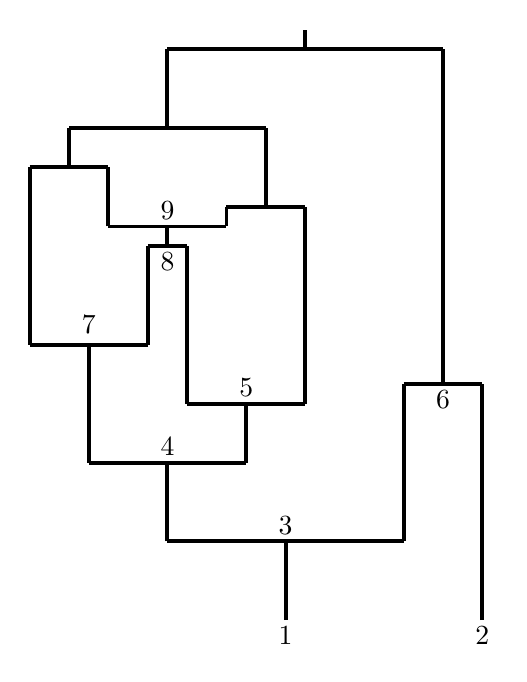
\begin{tikzpicture}
        \node[] at (0,-0.2) (1){1};
        \node[] at (2.5,-0.2) (2){2};
        \node[] at (0,1.2) (3){3};
        \node[] at (-1.5,2.2) (4){4};
        \node[] at (-0.5,2.95) (5){5};
        \node[] at (2,2.8) (6){6};
        \node[] at (-2.5,3.75) (7){7};
        \node[] at (-1.5,4.55) (8){8};
        \node[] at (-1.5,5.2) (9){9};
        
        \draw[-,black,line width=0.5mm] (0,0) -- (0,1); %1-3
        \draw[-,black,line width=0.5mm] (0,1) -- (-1.5,1); %3-4
        \draw[-,black,line width=0.5mm] (0,1) -- (1.5,1); %3-6
        \draw[-,black,line width=0.5mm] (1.5,1) -- (1.5,3); %3-6
        \draw[-,black,line width=0.5mm] (-1.5,1) -- (-1.5,2); %3-4
        \draw[-,black,line width=0.5mm] (-1.5,2) -- (-0.5,2); %4-5
        \draw[-,black,line width=0.5mm] (-1.5,2) -- (-2.5,2); %4-7
        \draw[-,black,line width=0.5mm] (-0.5,2) -- (-0.5,2.75); %4-5
        \draw[-,black,line width=0.5mm] (-2.5,2) -- (-2.5,3.5); %4-7
        \draw[-,black,line width=0.5mm] (-0.5,2.75) -- (-1.25,2.75); %5-8
        \draw[-,black,line width=0.5mm] (-0.5,2.75) -- (0.25,2.75); %5-10
        \draw[-,black,line width=0.5mm] (-1.25,2.75) -- (-1.25,4.75); %5-8
        \draw[-,black,line width=0.5mm] (0.25,2.75) -- (0.25,5.25); %5-10
        \draw[-,black,line width=0.5mm] (-2.5,3.5) -- (-3.25,3.5); %7-11
        \draw[-,black,line width=0.5mm] (-2.5,3.5) -- (-1.75,3.5); %7-8
        \draw[-,black,line width=0.5mm] (-1.75,3.5) -- (-1.75, 4.75 ); %7-8 
        \draw[-,black,line width=0.5mm] (-3.25,3.5) -- (-3.25,5.75); %7-11
        \draw[-,black,line width=0.5mm] (-1.75,4.75) -- (-1.5,4.75); %7-8
        \draw[-,black,line width=0.5mm] (-1.25,4.75) -- (-1.5,4.75); %5-8
        \draw[-,black,line width=0.5mm] (-1.5,4.75) -- (-1.5,5); %8-9
        \draw[-,black,line width=0.5mm] (-1.5,5) -- (-0.75,5);
        \draw[-,black,line width=0.5mm] (-1.5,5) -- (-2.25,5);
        \draw[-,black,line width=0.5mm] (-0.75,5) -- (-0.75,5.25);
        \draw[-,black,line width=0.5mm] (-0.75,5.25) -- (-0.25,5.25);
        \draw[-,black,line width=0.5mm] (0.25,5.25) -- (-0.25,5.25);
        \draw[-,black,line width=0.5mm] (-0.25,5.25) -- (-0.25,6.25);
        \draw[-,black,line width=0.5mm] (-2.25,5) -- (-2.25,5.75);
        \draw[-,black,line width=0.5mm] (-2.25,5.75) -- (-2.75,5.75);
        \draw[-,black,line width=0.5mm] (-3.25,5.75) -- (-2.75,5.75);
        \draw[-,black,line width=0.5mm] (-2.75,5.75) -- (-2.75,6.25);
        \draw[-,black,line width=0.5mm] (-2.75,6.25) -- (-0.25,6.25);
        \draw[-,black,line width=0.5mm] (-1.5,6.25) -- (-1.5,7.25);
        \draw[-,black,line width=0.5mm] (1.5,3) -- (2.5,3);
        \draw[-,black,line width=0.5mm] (2.5,0) -- (2.5,3);
        \draw[-,black,line width=0.5mm] (2,3) -- (2,7.25);
        \draw[-,black,line width=0.5mm] (2,7.25) -- (-1.5,7.25);
        \draw[-,black,line width=0.5mm] (0.25,7.25) -- (0.25,7.5);
    \end{tikzpicture}
    \caption{Caption}
    \label{fig:my_label}
\end{figure}



\begin{enumerate}
    \item Summary of Results 

    \item Applications of locating recombination nodes 
    \begin{enumerate}
        \item More precise location estimate (accuracy?)
        \item Where did populations meet history (Human History, Conservation)
        \item Key recombinants in co-infectiong in virus 
    \end{enumerate}
    
    \begin{enumerate}
        \item Compare dispersal estimates and location estimates to Brownian Motion
        \item Predict how they might alter estimates
        \item BM good for trees but not for ARGs. 
    \end{enumerate}
        
    \item Extension
    \begin{enumerate}
        \item Alternative spatial processes to brownian motion. 
        \item Non-symmetric movement (OU model)
        \item Habitat Boundaries 
        \item Epochs (Temporal heterogenity) 
        \item Spatial heterogenity in dispersal rates
    \end{enumerate}
    \item Future details Application of Datasets 
    \begin{enumerate}
        \item Simplification steps 
        \item Importance Sampling 
        \item Uncertainity in inference timings of recombination nodes. 
    \end{enumerate}
\end{enumerate}





\textbf{Bias in the Estimators}\\
We can find the bias in the MLE estimates by treating the MLEs as random variables dependent on the distribution of sample locations under the model, 
\begin{eqnarray}
    \widehat{\muvec} &=& \big( [\Rp,\Pp] [\Pp, \Pp]^{-1}[\Pp,\Rp] \big)^{-1} [\Rp,\Pp]\Lvec \\
    \widehat{\muvec_\ell} &=& [\Pp,\Pp]^{-1}[\Pp,\Rp]\widehat{\muvec} = \mathbf{B} \Lvec \\
    \widehat{\sigma^2} &=& \displaystyle \frac{(\Lvec - \widehat{\muvec_\ell})^\trp \smat^{-1}(\Lvec-\widehat{\muvec_\ell})}{n}
\end{eqnarray}
where $\mathbf{B} = [\Pp,\Pp]^{-1}[\Pp,\Rp]\big( [\Rp,\Pp] [\Pp, \Pp]^{-1}[\Pp,\Rp] \big)^{-1} [\Rp,\Pp] $ and $\Lvec$ is distributed normally as in Eq $\ref{eqn:Ldist}$. Therefore, we have 
\begin{eqnarray}
    E[\ \widehat{\muvec}\ ] &=& \big( [\Rp,\Pp] [\Pp, \Pp]^{-1}[\Pp,\Rp] \big)^{-1} [\Rp,\Pp]E[\Lvec] \\
    &=& \big( [\Rp,\Pp] [\Pp, \Pp]^{-1}[\Pp,\Rp] \big)^{-1} [\Rp,\Pp][\Pp,\Pp]^{-1}[\Pp,\Rp]\muvec\\
    &=& \muvec    
\end{eqnarray}
and, similarly, $E[\ \widehat{\muvec_\ell}\ ] = \muvec_\ell$, meaning no bias in the MLE estimates of the root locations.
Taking the expectation of MLE dispersal rate shows that
\begin{eqnarray}
    nE[\ \widehat{\sigma^2} \ ] &=& E[ \ \Lvec^\trp\smat^{-1}\Lvec -2\muvec_\ell^\trp \smat^{-1}\Lvec + \muvec_\ell^\trp \smat^{-1} \muvec_\ell \ ] \\
    &=& E[ \ \Lvec^\trp\smat^{-1}\Lvec \ ] + E[ \ -2\Lvec^\trp \mathbf{B}^\trp\smat^{-1}\Lvec + \Lvec^\trp \mathbf{B}^\trp \smat^{-1} \mathbf{B}\Lvec \ ] \\
    &=& E[ \ \Lvec^\trp\smat^{-1}\Lvec \ ] - E[ \ \Lvec^\trp \mathbf{B}^\trp\smat^{-1}\Lvec \ ] \\
    &=& \text{Trace}[ \smat^{-1} (\sigma^2 \smat) ] + \muvec_\ell^\trp \smat^{-1}\muvec_\ell -  \text{Trace}[  \mathbf{B}^\trp \smat^{-1} (\sigma^2 \smat) ]  - \muvec_\ell^\trp \mathbf{B}^\trp \smat^{-1}\muvec_\ell \\
    &=& \sigma^2 \text{Trace}[ \smat \smat^{-1} - \mathbf{B}^\trp ] + \muvec^\trp \mathbf{B}^\trp \smat^{-1} \mathbf{B} \muvec - \muvec^\trp \mathbf{B}^\trp \mathbf{B}^\trp \smat^{-1} \mathbf{B} \muvec \\
    &=& \sigma^2\text{Trace}[\mathbf{I}_n - \mathbf{B}^\trp] \\
    &=& \sigma^2(n - \text{Trace}[\mathbf{B}])
\end{eqnarray}
This implies that $\widehat{\sigma^2}$ is a biased estimate of $\sigma^2$, but that an unbiased estimate can be found by multiplying $\widehat{\sigma^2}$ by $n/(n-\text{Trace}[\mathbf{B}])$. Interestingly, in contrast to a tree (where $\text{Trace}[\mathbf{B}]=1$), in an ARG the bias appears to depend on both the topology (through $\Rp$ and $\Pp$) and the branch lengths (through $\spath$).
Note that above we have used $\mathbf{B}^\trp \smat^{-1} \mathbf{B} = \mathbf{B}^\trp\smat^{-1}$, $\mathbf{B}^2 = \mathbf{B}$ and $E[\vec{X}^\trp \mathbf{M} \vec{Y} ] = \text{Trace}[\Cov(\vec{Y},\vec{X})\mathbf{M}] + E[\vec{X}]^\trp\mathbf{X}E[\vec{Y}] $. The following is a proof of the latter,
\begin{eqnarray}
    E[\vec{X}^\trp \mathbf{M} \vec{Y} ] &=& \sum_{i=1}^{n_x} \sum_{j = 1}^{y_n} E[x_im_{ij}y_j] \\
    &=& \sum_{i=1}^{n_x} \sum_{j = 1}^{y_n} m_{ij}E[x_iy_j] \\
    &=& \sum_{i=1}^{n_x} \sum_{j = 1}^{y_n} m_{ij}\Big( \Cov(x_i,y_j) + E[x_i]E[y_j]\Big) \\
    &=& \sum_{i=1}^{n_x} \sum_{j = 1}^{y_n} m_{ij} \Cov(x_i,y_j) + \sum_{i}^{n_x} \sum_{j = 1}^{y_n} E[x_i]m_{ij}E[y_j] \\
    &=& \sum_{i=1}^{n_x} \sum_{j = 1}^{y_n} m_{ij} \Cov(y_j,x_i) + E[\vec{X}] \mathbf{M} E[\vec{Y }] \\
    &=& \sum_{i=1}^{n_x} \Big(\mathbf{M}\Cov(\vec{X},\vec{Y})\Big)_{ii}+ E[\vec{X}] \mathbf{M} E[\vec{Y }] \\
    &=& \text{Trace}[\mathbf{M}\Cov(\vec{X},\vec{Y})] + E[\vec{X}] \mathbf{M} E[\vec{Y }]
\end{eqnarray}


\section{Methods - Old}

To infer dispersal rates and ancestral locations using a maximum likelihood approach, we first assume that we have access to a time-calibrated ARG with marked recombination nodes (referred to as a "full" ARG in the {\tt msprime} and {\tt tskit} Python packages). An ARG is a directed acyclic graph with nodes representing haploid genomes (or a chromosome). Each edge extends from a "parent" (ancestral) node to a "child" node, describing a line of inheritance. Similarly to a tree, root and sample nodes are found top and bottom of the ARG, respectively. In many of the figures that we present, we focus on bifurcating ARGs, though our methods will work for more complex graphs. In these simpler scenarios, coalescent nodes have one parent node and two child nodes and recombination nodes have two parent nodes and one child node. Time is measured backwards starting from the present, with sample nodes at time $t=0$ and time increasing as we go deeper into the past to the root(s).

We model the movement of genetic material across generations, forward in time, by a Brownian motion with dispersal rate $\sigma^2$. In other words, we assume that the location of an offspring is normally distributed around one of its parent's locations with variance $\sigma^2$. While the computations are shown for working in one dimension, they can be extended to two dimensions by replacing the dispersal rate $\sigma^2$ with a dispersal matrix $\Sigma = \begin{bmatrix} 
    \sigma_x^2 & \sigma_{xy} \\
    \sigma_{xy} & \sigma_y^2
\end{bmatrix}$.

Similar methods have previously been applied to sparsely sampled, independent trees along the genome \citep{Osmond2021}, though as we explain below, extending these methods from a tree to a graph is non-trivial.

\subsection{Problem of Loops}

The locations of the samples under a model of Brownian motion have a multivariate normal distribution. When the genealogy is a tree, the covariance matrix is given by $\sigma^2 \mathbf{S}$, where $\mathbf{S}$ is a matrix whose $ij^{\text{th}}$ entry is the shared time between the paths from the root to the $i^{\text{th}}$ and $j^{\text{th}}$ sample. A key property that allows for the simple form of the covariance matrix is that the displacement along each edge of a tree under Brownian motion is independent from the displacement along every other edge. Therefore, the covariance between any two paths is given by $\sigma^2$ times the sum of the lengths of the shared edges between the paths. However for an ARG, the independence of displacements along edges doesn't hold. 

The main obstacle for calculating the likelihood of sample locations given a graph is the existence of loops. A loop in an ARG is characterized by two paths between a recombination node and a coalescence node that share no edges. These two paths must start and end in the same locations; this would be highly unlikely if we assume that the displacements along the edges are indeed independent and distributed $\cN(0,\sigma^2 t_{edge})$, where $t_{edge}$ is the length of the edge. For instance, in Fig \ref{fig:Method}, the displacement of the edge $5\rightarrow3$ must be equal to the sum of the displacements along the path $5 \rightarrow 4 \rightarrow 3$, as both start at node $5$ and end at node $3$.

\begin{figure}[h]
    \centering
    \includegraphics[width=\linewidth]{Images/Method_Outline.jpg}
    \caption{Outline of Paths Method. (A) A simple ARG (B) overlaying a Brownian motion on the ARG. (C) The shared time matrix for the paths in the ARG, $\spath$. \mo{would be nice to include the $\Pp$ matrix too}}
    \label{fig:Method}
\end{figure}

To derive the likelihood of sample locations under the ARG, denote the conditions imposed by loops in a full-ARG as $\eta_{loops}$ and let $\Lpvec$ be the vector of the locations of every path from the root to the samples, under the assumption of independence of edge displacements. This is a vector of length $p$, the number of paths from any sample to the root. The distribution of $\Lpvec$ is given, similar to the case of trees, by
\begin{eqnarray}
\Lpvec \sim \cN(\mu \onevec{p},\sigma^2 \spath )
\end{eqnarray}
where $\mu$ is the location of the root node, $\onevec{p}$ is a vector of ones of length $p$, and $\spath$ is a $p\times p$ matrix of shared times between paths (Fig \ref{fig:Method}). Here, the location of a sample node is not uniquely defined if there are multiple paths from the node to the root (i.e., if there are loops). We are interested in computing the distribution of the sample node locations, $\Lvec$, a vector of length $n$ (number of samples). This can be obtained by conditioning $\Lpvec$ on the loop conditions 
\begin{eqnarray}
    p_{\Lvec} (\lvec) = p_{\Lpvec | \eta_{loops}}(\Pp\lvec),
\end{eqnarray}
where $p_*$ is the probability density function of $*$ and $\Pp$ is a conversion matrix (see Notations for def) such that $\Pp \lvec$ is a vector of length $p$ associating to each path the location of the sample it corresponds to. 

\subsection{Solution of Paths}

While it is possible to get the conditional distribution $\Lpvec | \eta_{loops}$ (see Appendix \ref{}), it isn't straightforward to develop an algorithm to do so. However, there is an equivalent method which is more computationally feasible.

Instead of focusing on the loops, we identify the paths through the ARG that go from a root node to a sample node. Unlike genealogical trees, where the number of paths is always equal to the number of samples, the number of paths through an ARG grows with the number of recombination nodes ($r$) within the graph. The displacements along these paths must meet the condition that all paths that start at the same root node and end at the same sample node must have the same total displacement; we define this condition as $\eta_{paths}$. While this condition is distinct from $\eta_{loops}$ (e.g.,  in Fig \ref{fig:Method} this is 3$\rightarrow$5 = 3$\rightarrow$4$\rightarrow$5), which only involves edges in a recombination loop, they are indeed equivalent, i.e. $\eta_{loops} = \eta_{paths}$ (see Appendix \ref{} for a general proof). Importantly, we could identify every single path through the ARG, but many of the paths are not linearly independent from one another and therefore are redundant in our calculations. We denote the minimal set of paths through the ARG that still satisfies the conditions of $\eta{loops}$; the size of this set ($p$) is equal to $n+r$.

The distribution of the sample locations can be found by conditioning the path locations, $\Lpvec$ on $\eta_{paths}$, instead of on $\eta_{loops}$, giving
\begin{equation}
\Lvec \sim \cN(\mu \onevec{n},\sigma^2 \mathbf{S} ),
\end{equation}
where $\mathbf{S} = \sigma^2 (\Pp^T\spathg\Pp)^{-1} $. Here, $\spathg$ is the Moore-Penrose generalized inverse of $\spath$, since $\spath$ may not be invertible as different paths before conditioning need not be linearly independent. 

\subsection{Algorithm}

\begin{figure}[htp]
    \centering
    \includegraphics[width=12cm]{Images/algorithm.png}
    \caption{Visualization of the optimized algorithm. Given a hypothetical ARG of three samples (left) with four paths, the algorithm builds the covariance matrix by looping through the nodes in the ARG. Within the looping block, the bolded numbers in each matrix are those that were updated in that specific step.}
    \label{fig:algorithm}
\end{figure}

The key object for computing dispersal rates and node locations is the matrix of shared time between minimal set of paths through the ARG, $\spath$. Though there are existing methods in {\tt Python} to identify paths from the samples to the GMRCA, calculating the intersection between these paths doesn't scale well to larger ARGs primarily due to repeated calculation of common edges between different paths (Fig \ref{fig:AlgorithmEff}). We have developed an algorithm that requires traversing each edge only once and in doing so have greatly sped up this process of identifying and comparing the minimal set of paths in the ARG (Fig \ref{fig:AlgorithmEff}). 

Briefly, the algorithm entails an bottom-up traversal of the ARG starting at the sample nodes and updating the shared time matrix as we traverse upwards towards the roots (Fig \ref{fig:algorithm}). For each node visited, the algorithm calculates the edge length between that node and its parent. This is added to the corresponding cells in the shared time matrix. When the node visits a recombination node (which have multiple parents), the relevant rows and columns are also duplicated, expanding the size of the matrix and corresponding with the separation of these paths in the ARG. This keeps the size of the matrix smaller for as long as possible, making it more efficient. For a step-by-step implementation of the algorithm, see Appendix \ref{appedix:ch2}.

\begin{figure}[h]
    \centering
    \includegraphics[width=0.45 \linewidth]{Images/benchmark_small.png}
    \caption{Benchmarking for the time that it took the each method to calculate the shared time matrices, $\spath$, for a set of random ARGs generated by the msprime Python package \citep{Baumdicker2022}. More details on the parameters passed to msprime can be found in the Supplementary. All algorithms were run on the same set of ARGs, and for each ARG, the algorithm that went first was chosen at random to minimize any unintended biases associated with the ordering of the algorithms.}
    \label{fig:AlgorithmEff}
\end{figure}



\subsection{Maximum likelihood estimates of root location and dispersal rate}

Similar to the case of trees, the maximum likelihood estimates of the root location and dispersal rate are
\begin{eqnarray}
    \muMLE &=& (\onevec{n}^\text{T} \sinv \onevec{n})^{-1}(\onevec{n}^\text{T} \sinv \ldata) = (\onevec{p}^\text{T} \spathg \onevec{p})^{-1}(\onevec{p}^\text{T}\spathg\Pp \ldata) \\
    \sigmaMLE &=& \displaystyle \frac{ (\ldata - \muMLE\onevec{p})^\text{T} \Pp^\text{T}\spathg\Pp (\ldata - \muMLE\onevec{p}) }{n}
\end{eqnarray}
where $\ldata$ are the observed sample locations. $\sigmaMLE$ is a biased estimator since it depends on the estimate of the root location $\muMLE$, which has uncertainty associated with it. We can correct this bias by multiplying $\sigmaMLE$ by $n/(n-1)$.


\subsection{Multiple roots}


There are many reasons why we might want to focus on just the recent past in our analysis. Firstly, long term dispersal patterns may not be accurately captured by our Brownian motion model, particularly in the presence of geographic barriers to dispersal or directional population movements \citep{Ianni2022, WakeleySCATTERINGETC}. Secondly, as we move further back into the past, sample lineages can become spatially well mixed. Therefore, it becomes difficult or impossible to extract any meaningful spatial information about the deep history of samples. Lastly with ARG inference, deeper nodes in the ARG are often poorly resolved, both in timing and topology. To account for this, we may want to cutoff the ARG at a given time in the past and ignore any deeper connections.

When we chop an ARG, the graph no longer has a GMRCA and instead has multiple roots, each associated with specific paths through the ARG. Let $\vec{\mu}$ be the vector of root locations (of length $r$) and $\Rp \mu$ be the vector associating each path to its corresponding root (of length $p$). Here, $R_p$ is be a conversion matrix of size $p \times r$, where $r$ is the number of roots in the tree sequence. The $i,j^{th}$ element of $R_p$ has value 1 if path $j$ terminates at root $i$, otherwise this element has value 0.


Since the assumption of unbounded motion doesn't hold in the deeper past due to finite habitats \citep{Ianni2022, WakeleySCATTERINGETC} and inference until the GMRCA isn't usually desirable or possible from the sequence data \cite{}, we will often want to cut off an ARG some time in the past. 
Doing this will often result in the ARG having multiple roots, which hasn't been accounted for above. Let $\vec{\mu}$ be the vector of root locations (of length $r$) and $\Rp \mu$ be the vector associating each path to its corresponding root (of length $p$). Here, $\Rp$ is a conversion matrix of size $p \times r$, where the position $i,j$ in $\Rp$ has value 1 if path $i$ contains root $j$, and 0 otherwise. 

In this case, the full covariance between the paths is the covariance within the ARG plus the covariance between the root locations, $\sigma^2 ( \spath + \text{Cov}(\Rp\muvec, \Rp\muvec)) $. However, we assume that the root locations are independent of each other and constant, causing $\text{Cov}(\Rp\muvec, \Rp\muvec)=0$. The assumption of independence is reasonable if we cut off the trees at a point by which the ancestors are well mixed in a finite habitat. The assumption of constant root locations can be relaxed by adding the correct variance to the covariance term between paths starting at the same root. 

We can then compute the maximum likelihood estimate for the root locations given the sample locations, $\ldata$, as a solution to the following system of linear equations

\begin{eqnarray}
    \label{eq:location_of_roots}
    \Rp^\text{T}\spathg\Rp  \muvecMLE = \Rp\spathg\Pp\ldata  
\end{eqnarray}

If $\Rp^\text{T}\spathg\Rp$ is invertible (NOTE: Haven't proved it but I think this should always be invertible), then there exists a unique solution,
\begin{eqnarray}
 \muvecMLE = (\Rp^\text{T}\spathg\Rp)^{-1} \Rp\spathg\Pp\ldata   
\end{eqnarray}
which is a generalized version of $\muMLE$ for a single root (above) and reduces to the same when there is a single root ($\Rp = \onevec{p}$).

Once we have the roots, we can compute the unbiased estimator for the dispersal rate 
\begin{eqnarray}
    \sigmaMLE &=& \displaystyle \frac{ (\Pp\ldata - \Rp\muvecMLE)^\text{T} \spathg (\Pp\ldata - \Rp\muvecMLE) }{n-k}.
\end{eqnarray}
where $k = \text{trace}[  \Pp^\text{T}\spathg\Rp(\Rp^\text{T}\spathg\Rp)^{-1}\Rp^\text{T}\spathg\Pp(\Pp^\text{T}\spathg\Pp)^{-1} ]$ . The $n-k$ is the correction for the bias in the Maximum Likelihood Estimator (See Appendix \ref{}), which depends on the topology and branch lengths of the ARG. When there is a single root ($\Rp = \onevec{p}$) then $k=1$ (as in the case of an ARG with a single root, above).

\subsection{Internal Node Locations}
  

Once we have estimates of the dispersal rate and root locations we can get the distribution of internal node locations as well. Given an internal node, $a$, its location, $\Lint$, is distributed as
\begin{eqnarray}
    \Lint | \muvecMLE, \sigmaMLE, \ldata \sim \cN \bigg( \muMLE_a + \savec^\text{T}\spathg(\Pp\ldata - \Rp \muvecMLE), \sigmaMLE(t_a - \savec^\text{T}\spathg\savec)\bigg)
\end{eqnarray}
conditional on the dispersal rate, root locations, and observed sample locations. However, since the root locations have associated uncertainty, one can use the law of total variance to find the complete variance,
\begin{eqnarray}
    \Var \Lint = \sigmaMLE\left(t_a - \savec^\text{T}\spathg\savec + \displaystyle \frac{(1 - \savec^\text{T}\spathg\onevec{p})^2}{\onevec{p}^\text{T}\spathg\onevec{p}}\right).
\end{eqnarray}
\mo{say something about what this means, or that it is just analagous to the case of trees}



\subsection*{Spatially-explicit simulations}

We performed spatial simulations using SLiM v4 \citep{haller_slim_2023}, extending those run by \citet{osmond_estimating_2021}. Simulations had a starting population of 10,000 individuals, with each individual being diploid for a 1 megabase chromosome. Individuals were uniformly randomly distributed in a $100 \times 100$ unit area. Each tick in the simulations corresponds with a generation. Individuals reproduce based on conditions in their local neighborhood; all individuals are hermaphrodites and mates are chosen randomly based on their distance to the focal individual. The number of offspring is a Poisson random variable with $\lambda=\frac{2}{1 + C}$, where C is the sum of the interaction strengths with neighbors (Beverton-Holt model of density dependence with average number of offspring = 2 and local carrying capacity = 1). It is possible that there aren't any mates within the interaction distance; in these cases, no offspring are produced. Offspring are placed close to one of their parents positions with an normal random variable offset in each dimension; the variance of this offset is the dispersal rate. The area has reflecting boundaries; if this offset would place the offspring outside of the area, the offset is reflected off of the boundary wall and back into the area. The positions and relationships between individuals are recorded in a tree sequence, which is saved at the end of the simulation (for more information about the recording process, see \citet{haller_tree-sequence_2019}).

